%% Copyright 2022 P. S. Eduardo.
%
% This work may be distributed and/or modified under the
% conditions of the LaTeX Project Public License, either version 1.3
% of this license or (at your option) any later version.
% 
% The Current Maintainer of this work is P. S. Eduardo.
%
% This work consists of the file poliStyles.sty.
%% -----------------------------------------------------------------
% Escola Politécnica UFRJ LaTeX Template
% Version: 2209
%                   Eduardo Paiva dos Santos
%email: eduardopaiva@poli.ufrj.br
%%------------------------------------------------------------------

\documentclass[handout,10pt,aspectratio=169]{beamer}

\usepackage{style/poliStyles}
\usepackage{style/tensorOperator}

\setlength{\columnsep}{3cm}

% Definições de comandos e ambientes customizados: uso opcional
% -----------------------------------------------------------------------------------
% Comandos auxiliares
% -----------------------------------------------------------------------------------
\newcommand{\slideTitle}[1]{\frametitle{\textbf{#1}}}
\newcommand{\itemb}{\item[$\bullet$]}
\newcommand{\code}[1]{\texttt{#1}}
\newcommand{\bfcode}[1]{\texttt{\textbf{#1}}}
\newcommand{\bash}[1]{\code{\$> #1 }}
\newcommand{\direct}[1]{{\textbf{\code{#1}}}}
\newcommand{\PR}[1]{\ensuremath{\left[#1\right]}}
\newcommand{\PC}[1]{\ensuremath{\left(#1\right)}}
\newcommand{\chav}[1]{\ensuremath{\left\{#1\right\}}}

\newcommand{\info}[1]{
\includegraphics[#1]{figures/icons/information} \hspace{0.1cm}}
\newcommand{\warn}[1]{
\includegraphics[#1]{figures/icons/warning} \hspace{0.1cm}}
\newcommand\at[2]{\left.#1\right|_{#2}}

%% -----------------------------------------------------------------------------------------------
% % Importando APUD do abntcite.sty
\RequirePackage{ifthen}
\def\citeopen{(}
\def\citeclose{)}
\renewcommand{\apud}[3][]{\citeopen\citeauthor{#2}, \citeyear{#2} \apudname\ %
\citeauthor{#3}, \citeyear{#3}%
\ifthenelse{\equal{#1}{\empty}}{}{, #1}\citeclose}

\renewcommand{\apudonline}[3][]{\citeonline{#2} \apudname\ %
\citeonline{#3}%
\ifthenelse{\equal{#1}{\empty}}{}{, #1}}
%% -----------------------------------------------------------------------------------------------

% -----------------------------------------------------------------------------------
% Comandos para citacao de softwares
% -----------------------------------------------------------------------------------
\newcommand{\pointwise}{\href{http://pointwise.com/}{\code{Pointwise}} }
\newcommand{\cfMesh}{\href{http://cfmesh.com/}{\code{cfMesh}} }
\newcommand{\salome}{\href{http://www.salome-platform.org/}{\code{Salome}} }
\newcommand{\OpenFOAM}{\href{http://www.openfoam.org/}{\code{OpenFOAM}} }
\newcommand{\foamExtend}{\href{http://www.extend-project.de/}{\code{foam-extend}} }
\newcommand{\paraview}{\href{http://www.paraview.org/}{\code{ParaView}} }


% -----------------------------------------------------------------------------------
% Definicao do ambiente slide e slideWithFrameBreaks
% -----------------------------------------------------------------------------------
\newenvironment{slide}[1]
{
    \begin{frame}
        \slideTitle{#1}
        \vfill
}
{
        \vfill
    \end{frame}
}

\newenvironment{slideWithCode}[1]
{
    \begin{frame}[fragile, environment=slideWithCode]\slideTitle{#1}
    \vfill
}
{
    \vfill
    \end{frame}
}

\newenvironment{slideWithFrameBreaks}[1]
{
    \begin{frame}[allowframebreaks]{\textbf{#1}}
}
{
    \end{frame}
}

\newenvironment{slideWithFrameBreaksWithCode}[1]
{
    \begin{frame}[fragile, environment=slideWithFrameBreaksWithCode, allowframebreaks]{\textbf{#1}}
}
{
    \end{frame}
}

% \newenvironment{slideWithFrameBreaksWithCode}[1]
% {
%     \begin{frame}[fragile][allowframebreaks]{\textbf{#1}}
% }
% {
%     \end{frame}
% }
% -----------------------------------------------------------------------------------

% -----------------------------------------------------------------------------------
%  Redefinicao dos ambientes enumarate e itemize, com espacamentos diferenciados
% -----------------------------------------------------------------------------------
% \newenvironment{cmd}[args][default]{beginDef}{endDef}
\newenvironment{Enum}[1][0.25]
{
    \begin{enumerate}
        \itsep{#1}
        \setlength{\parskip}{0pt}
        \setlength{\parsep}{0pt}
}
{
    \end{enumerate}
}

\newenvironment{Item}[1][0.25]
{
    \begin{itemize}
        \itsep{#1}
        \setlength{\parskip}{0pt}
        \setlength{\parsep}{0pt}
}
{
    \end{itemize}
}

%%--------------------------------------------------------------------------------------------------
% Definição de slide com margem diferenciada: usado para slides de transição; início das seções
%% -------------------------------------------------------------------------------------------------

\NewEnviron{wideframe}[1][]
{
    \begin{frame}{#1}
        \vfill
        \makebox[\textwidth][c]
        {
            \begin{minipage}{\dimexpr\paperwidth-\MARGIN-\MARGIN\relax}
                \BODY
            \end{minipage}
        }
        \vfill
    \end{frame}
}

%% -------------------------------------------------------------------------------------
% Customizacao de boxes do pacote tcolorbox
%% --------------------------------------------------------------------------------------------

\newenvironment{myBox}[1][]
{
    \begin{tcolorbox}
    [
        colback=gray!20!white,
        colbacktitle=poliBlue!70!black,
        coltitle=white,
        colframe=poliBlue!70!black,
        boxrule=2pt,
        titlerule=4pt,
        arc=0pt,
        boxsep=2pt
    ]
}
{
    \end{tcolorbox}
}

\newenvironment{objectiveBox}[1][]
{
    \begin{tcolorbox}
    % [
    %     colback=gray!30!white,
    %     colbacktitle=poliBlue!70!black,
    %     coltitle=white,
    %     colframe=gray!30!white,
    %     boxrule=2pt,
    %     titlerule=4pt,
    %     arc=0pt,
    %     boxsep=2pt,
    %     width=#1
    % ]
}
{
    \end{tcolorbox}
}

\newenvironment{myBox2}[1][\linewidth]
{
    \begin{tcolorbox}
    [
        colback=gray!30!white,
        colbacktitle=poliBlue!70!black,
        coltitle=white,
        colframe=poliBlue!70!black,
        boxrule=2pt,
        titlerule=4pt,
        arc=0pt,
        boxsep=2pt,
        width=#1
    ]
}
{
    \end{tcolorbox}
}

\newenvironment{myCodeBox}[1][\linewidth]
{
    \begin{tcolorbox}
    [
        colback=white,
        colbacktitle=poliBlue!70!black,
        coltitle=white,
        colframe=poliBlue!70!black,
        boxrule=2pt,
        titlerule=4pt,
        arc=0pt,
        boxsep=2pt,
        width=#1
    ]
}
{
    \end{tcolorbox}
}

\newenvironment{myTitledBox}[1][Theorem:]
{
    \begin{tcolorbox}
    [
        colback=gray!20!white,
        colbacktitle=poliBlue!70!black,
        coltitle=white,
        colframe=poliBlue!70!black,
        boxrule=2pt,
        titlerule=4pt,
        arc=0pt,
        boxsep=2pt,
        title=#1
    ]
}
{
    \end{tcolorbox}
}

\newenvironment{myTitledBox2}[2]
{
    \begin{tcolorbox}
    [
        colback=gray!20!white,
        colbacktitle=poliBlue!70!black,
        coltitle=white,
        colframe=poliBlue!70!black,
        boxrule=2pt,
        titlerule=4pt,
        arc=0pt,
        boxsep=2pt,
        width=#1,
        title=#2
    ]
}
{
    \end{tcolorbox}
}

% \newenvironment{myTitledBox2}[1][Theorem:][.\textwidth]{%
%   \setlength{\textwidth}{#1}
% {
%     \begin{tcolorbox}
%     [
%         colback=gray!20!white,
%         colbacktitle=red!70!black,
%         coltitle=white,
%         colframe=red!70!black,
%         boxrule=2pt,
%         titlerule=4pt,
%         arc=0pt,
%         boxsep=2pt,
%         title=#1
%     ]
% }
% {
%     \end{tcolorbox}
% }

% \lstset
% {
%     backgroundcolor=\color{gray!20!white},  
%     basicstyle=\ttfamily \footnotesize, 
%     breakatwhitespace=false,
%     breaklines=true,
%     captionpos=b,
%     commentstyle=\color{gray},
%     deletekeywords={...},
%     escapeinside={\%*}{*)},
%     extendedchars=true,
%     frame=single,
%     keepspaces=true,
%     keywordstyle=\color{blue},
%     otherkeywords={*,...},
%     numbers=left,
%     numbersep=5pt,
%     numberstyle=\tiny \color{gray},
%     rulecolor=\color{red!70!black},
%     showspaces=false,
%     showstringspaces=false,
%     showtabs=false,
%     stepnumber=1,
%     stringstyle=\color{red},
%     tabsize=4,
%     title=\lstname
% }


%% -------------------------------------------------------------------------
% Título, autor e instituição
%% -------------------------------------------------------------------------


\title[Todos os direitos reservados]
{     
     \textbf{Projeto Final de Graduação}
}

\subtitle[]
{
    Título do Projeto
}

\author{Nome Completo}

\institute{Universidade Federal do Rio de Janeiro}

\date{\today}

%% -------------------------------------------------------------------------
% Índice da apresentação
%% -------------------------------------------------------------------------

% NOTA: Caso o número de sessões exceda o espaço, é recomendado utilizar a opção 2

% Opção 1
% \AtBeginSection[]{	
%   \begin{wideframe}
%     \frametitle{\textbf{Plano da Apresentação}}
%     \vfill
%     \setstretch{3.0}
%     \tableofcontents[currentsection]
%   \end{wideframe}
% }

% Opção 2
\AtBeginSection[]
{
  \begin{wideframe}
    \begin{multicols}{2}
    \setlength{\columnsep}{-0.5cm}
    \frametitle{\bf{Plano da Apresentação}}
        \vfill
        \setstretch{3.0}
        
        \tableofcontents[currentsection]
        \end{multicols}
    
  \end{wideframe}
}

%% -------------------------------------------------
% Objetivos desta apresentação
%% -------------------------------------------------


\begin{document}
\maketitle

\begin{slide}{Temas e Objetivos}

	\begin{objectiveBox}[\linewidth]
	\justifying
    	\textbf{Objetivo Principal:}
    	\begin{Item}
    	    \item Objetivo 1;
    	    \item Objetivo 2; 
        \end{Item}
	\end{objectiveBox}
	
    \begin{objectiveBox}[\linewidth]
    \justifying
    \textbf{Resultados Esperados:} 
        \begin{Item}
    	    \item Resultado 1;
    	    \item Resultado 2;
        \end{Item}
    \end{objectiveBox}	
	
\end{slide}

%% -------------------------------------------------
% Inclusão dos capítulos
%% -------------------------------------------------

    	\section{Introdução}
\begingroup\small

\begin{slide}{A Crise Global da Água}
  \begin{columns}
    \begin{column}{.55\linewidth}
      \begin{Item}
        \item 4 bilhões de pessoas enfrentam escassez severa $\ge$1 mês/ano (Mekonnen \& Hoekstra, 2016)
        \item 2,2 bilhões sem acesso a água potável segura (WHO, 2023)
        \item Demanda global deve superar oferta em 40\% até 2030 (IDRA, 2026)
      \end{Item}
    \end{column}
    \begin{column}{.45\linewidth}
      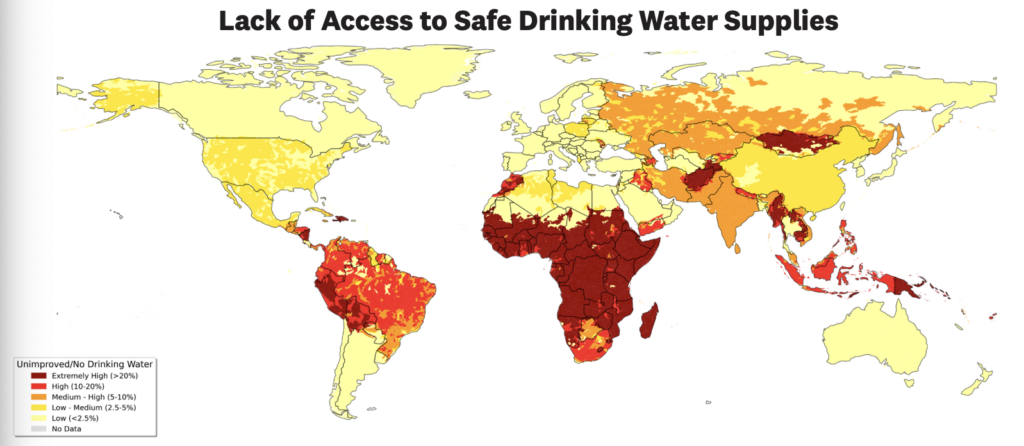
\includegraphics[width=\linewidth]{tcc_images/criseH.png}
    \end{column}
  \end{columns}
  \vfill\hfill{\scriptsize Fontes: WHO, 2023; IDRA, 2026; Imagem: Health Policy Watch, 2024}
  \note{A crise global da água é tanto de quantidade quanto de qualidade. 4 bilhões sofrem com escassez, 1,7 bilhão bebem água contaminada, causando mais de 500 mil mortes por ano. É um problema que demanda soluções urgentes e inovadoras. [~1 min]}
\end{slide}
%========================================================================

\begin{slide}{O Problema no Brasil}
  \begin{columns}[T]
    \begin{column}{.55\linewidth}
      \begin{Item}
        \item 2026: ano desafiador — chuvas abaixo da média; Cantareira $\approx$ 30\% (\textcolor{poliRed}{ANA} — Agência Nacional de Águas)
        \item Nordeste: 4 meses de chuva e 8 meses de seca extrema (ANA)
        \item Dessalinização: em ambientes de escassez, viabiliza desenvolvimento econômico e melhora a qualidade de vida via oferta de água de boa qualidade (estudo \textcolor{poliRed}{CNI}, 2026 \cite{CNI2026})
        \item Maior planta do Brasil (ES): atende demanda de 80 mil pessoas \cite{CNI2026}
        \item 8.500 km de costa $\rightarrow$ enorme potencial para expandir (IBGE)
      \end{Item}
    \end{column}
    \begin{column}{.45\linewidth}
      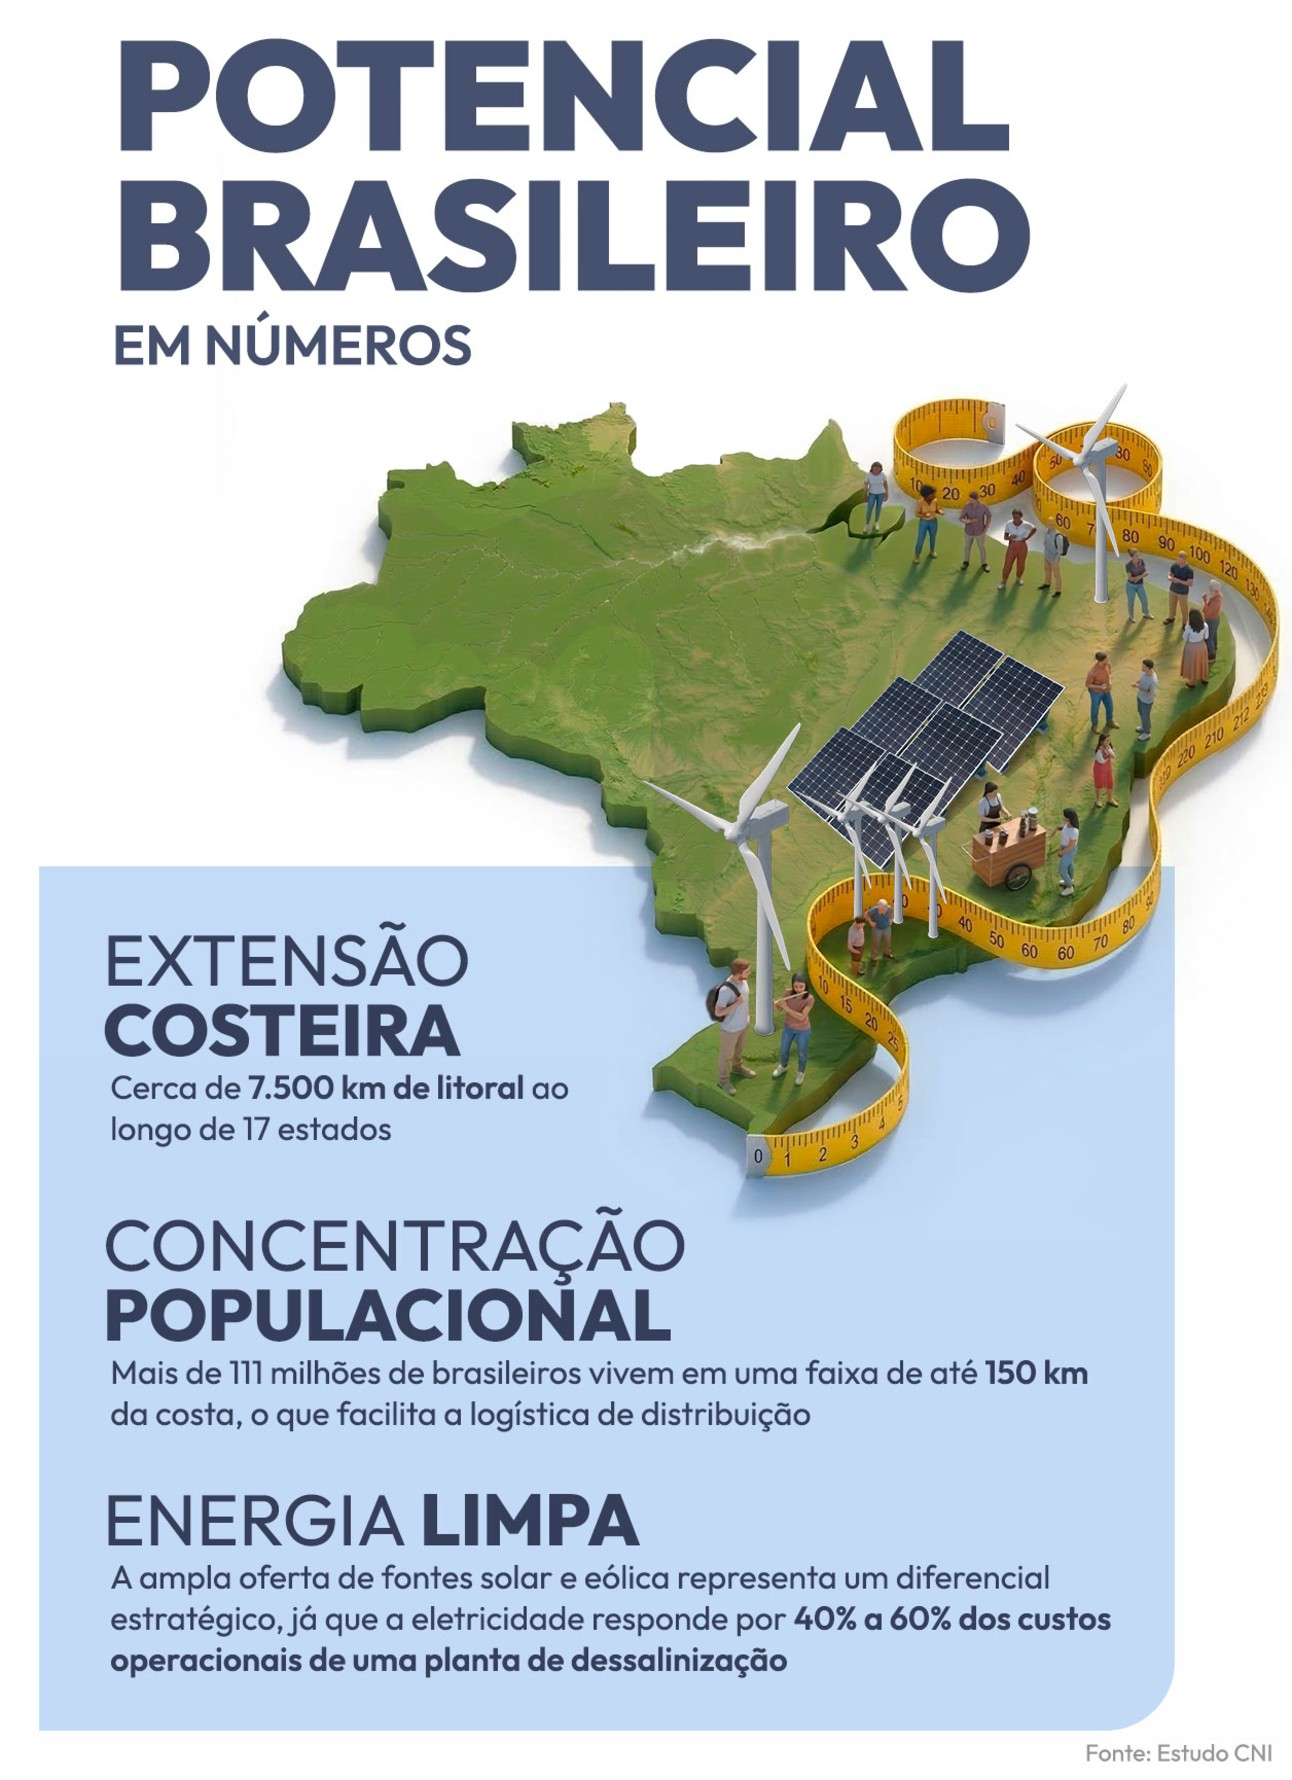
\includegraphics[width=\linewidth]{tcc_images/artebrasillet.jpg}
    \end{column}
  \end{columns}
  \vfill\hfill{\scriptsize Fontes: ANA, 2026; CNI, 2026 \cite{CNI2026}; IBGE; Imagem: CNI, 2026}
   \note{No Brasil, 2026 é desafiante para a gestão de água. O Cantareira está pouco acima de 30\%. No Nordeste, 4 meses de chuva contra 8 de seca extrema. A dessalinização desponta como alternativa estratégica para segurança hídrica segundo estudo da CNI. A maior planta do Brasil, no ES, atende 80 mil pessoas. Com 8.500 km de costa, o potencial de expansão é enorme. [~1 min]}
\end{slide}
%========================================================================

\begin{slide}{O V-AGMD no Contexto da Dessalinização}
  \small
  \begin{columns}
    \begin{column}{.55\linewidth}
      \begin{Item}
        \item \textbf{Dessalinização} divide-se em duas grandes tecnologias:
        \begin{Item}
          \item Processos \textbf{térmicos} (destilação convencional)
          \item Processos de \textbf{membrana} (osmose inversa, MD)
        \end{Item}
        \item \textbf{Destilação por Membrana (MD)}: processo térmico que utiliza uma membrana hidrofóbica para separar o vapor da água da salmoura aquecida
        \item \textcolor{poliRed}{\textbf{V-AGMD}}: configuração que combina \textbf{espaço de ar} (isolamento térmico) com \textbf{vácuo parcial} ($\rightarrow$ menor resistência à transferência de massa do vapor, acelerando o transporte) — foco deste trabalho
      \end{Item}
    \end{column}
    \begin{column}{.4\linewidth}
      \centering
      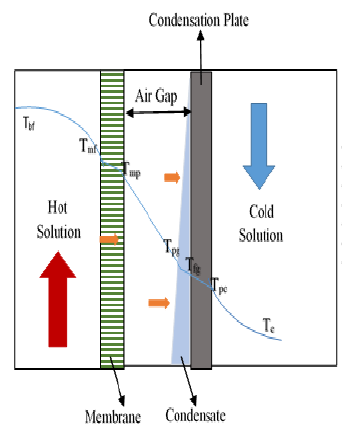
\includegraphics[width=0.85\linewidth]{tcc_images/chap03/Model-of-heat-and-mass-transfer-in-the-AGMD.png}\\[4pt]
      {\tiny Figura: Transporte de calor e massa na MD. Fonte: Zheng (2017)}
    \end{column}
  \end{columns}
  \note{A dessalinização se divide em térmicos e membrana. A MD é um processo térmico que utiliza uma membrana hidrofóbica para separar o vapor d'água. O V-AGMD combina espaço de ar com vácuo: o ar isola termicamente, o vácuo acelera o vapor. [~45s]}
\end{slide}
%========================================================================

\begin{slide}{Ilha de Policogeração Sustentável (LabMEMS/COPPE)}
  \begin{columns}
    \begin{column}{.5\linewidth}
      \begin{Item}
        \item Protótipo pioneiro COPPE/UFRJ (2022): água potável + energia via solar térmica
        \item 5 kW$_e$ ($\approx$ 25 residências) + 8 kW$_t$ recuperáveis em micro-trocadores
        \item Dessalinizador V-AGMD: produz 1.000 L/dia de água destilada ($>$ 100 pessoas/dia)
        \item Foco em comunidades remotas/off-grid (Semiárido, ilhas, O\&G, áreas de desastre)
        \item Potencial complementar a projetos existentes de dessalinização em locais de escassez, como o \textcolor{poliRed}{\textbf{Projeto Água Doce}} (programa federal para o Semiárido nordestino)
      \end{Item}
    \end{column}
    \begin{column}{.5\linewidth}
      \centering
      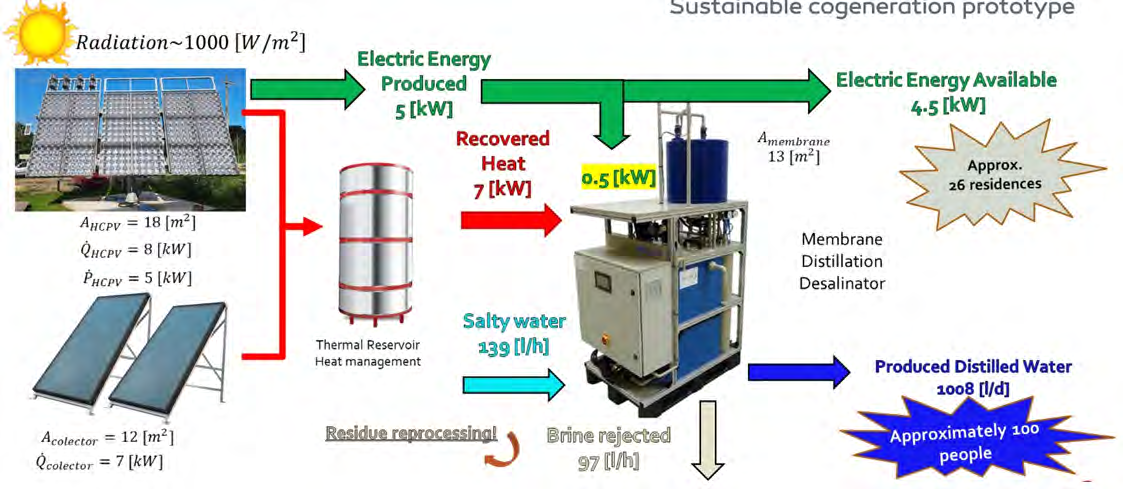
\includegraphics[width=\linewidth]{tcc_images/instalacao_ips.png}
    \end{column}
  \end{columns}
  \vfill\hfill{\scriptsize Fontes: COPPE/UFRJ, 2022; LISBOA et al., 2024; NAVEIRA-COTTA et al. [s.d.]}
  \note{A Ilha de Policogeração Sustentável da COPPE, inaugurada em 2022, é o projeto que abriga este trabalho. É um sistema que integra painéis solares de alta concentração com um dessalinizador V-AGMD, produzindo eletricidade para 25 residências e água para mais de 100 pessoas por dia. O foco são comunidades remotas. Potencial complementar ao Projeto Água Doce. [~1 min]}
\end{slide}
%========================================================================

% Slide da imagem sozinha removido — integrado ao slide anterior
% \begin{slide}{}
%   \vspace*{\fill}
%   \begin{center}
%     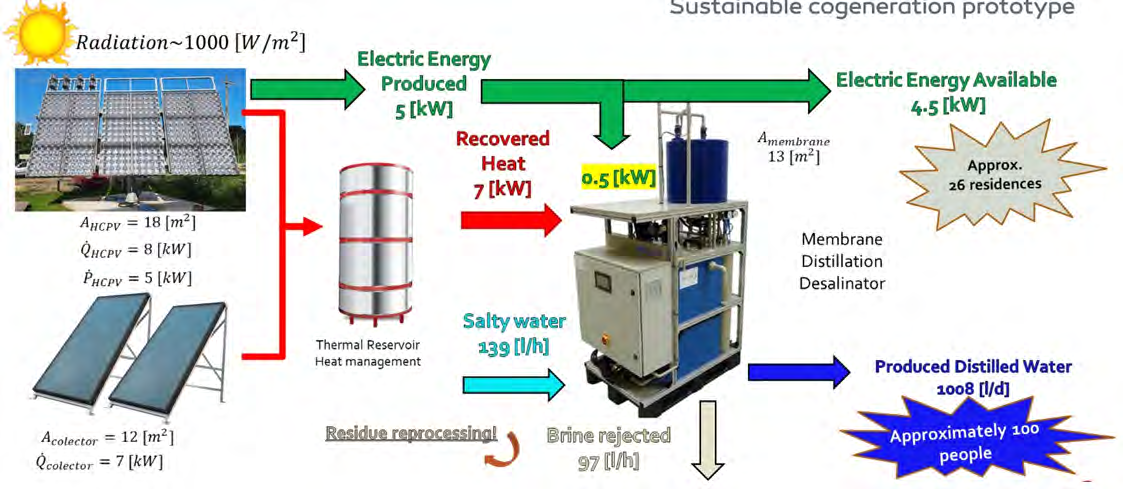
\includegraphics[width=0.9\textwidth, height=0.8\textheight, keepaspectratio]{tcc_images/instalacao_ips.png}
%   \end{center}
%   \vspace*{\fill}
%   \vfill\hfill{\scriptsize Fonte: NAVEIRA-COTTA et al. [s.d.]}
% \end{slide}
%========================================================================

\begin{slide}{Objetivos}
  \footnotesize
  \begin{myTitledBox}[Objetivos]
    \textbf{Objetivo geral:} avaliar e selecionar modelos de regressão supervisionada para predição do desempenho do módulo V-AGMD (fluxo de permeado e temperaturas de saída), combinando aprendizado a partir de dados experimentais (174 pontos, 3 regimes de salinidade) com informação física proveniente de um modelo reduzido 0D já publicado pelo laboratório (LISBOA et al., 2024).
  \end{myTitledBox}
  \note{Objetivo geral: avaliar e selecionar modelos de regressão supervisionada para predição do desempenho do V-AGMD, combinando dados experimentais (174 pontos, 3 regimes) com o modelo físico 0D do laboratório como referência. [~1 min]}
\end{slide}
%========================================================================

\nocite{Abid2020}
\nocite{Lisboa2024}
\endgroup

    	\section{Revisão Bibliográfica}

\begin{slide}{Abordagens de Modelagem em MD}
  \small
  \centering
  \resizebox{\textwidth}{!}{
    \begin{tabular}{p{0.18\linewidth} p{0.15\linewidth} p{0.32\linewidth} p{0.15\linewidth} p{0.17\linewidth}}
      \toprule
      \textbf{Abordagem} & \textbf{Tecnologia} & \textbf{Descrição} & \textbf{Vantagens} & \textbf{Limitações} \\
      \midrule
      \textbf{Física}
      & AGMD, 2D, \textbf{V-AGMD}
      & Modelos 0D, 1D, 2D
      & Interpretabilidade física
      & Custo computacional cresce com a complexidade (0D $\rightarrow$ 1D $\rightarrow$ 2D) \\
      \midrule
      \textbf{Dados}
      & \textbf{AGMD}, VMD
      & Técnicas de regressão (Ex: Redes Neurais) para predição de fluxo e temperaturas
      & Alta flexibilidade; aprox. não linear
      & Pouca interpretabilidade; generalizam bem com muitos dados e mal quando há escassez \\
      \midrule
      \textbf{Híbridos (físico + dados)}
      & DCMD, \textbf{V-AGMD}
      & Combinam modelos físicos reduzidos com técnicas de regressão
      & Combina física + dados; regulariza o espaço de busca
      & Complexidade de implementação \\
      \bottomrule
    \end{tabular}
  }
  \note{A revisão mostra três grandes abordagens para modelagem em MD. Física: interpretável mas cara — custo computacional cresce com a complexidade. Data-driven: flexível, mas com pouca interpretabilidade e generalização dependente do volume de dados. Híbridos: combinam o melhor dos dois mundos com maior complexidade de implementação. [~1,5 min]}
\end{slide}
%========================================================================

\begin{slide}{Panorama de Publicações em MD}
  \small
  \centering
  \begin{tabular}{p{0.22\linewidth} p{0.10\linewidth} p{0.55\linewidth}}
    \toprule
    \textbf{Abordagem} & \textbf{Nº} & \textbf{Modelos} \\
    \midrule
    \textbf{Física} & 4 & 0D, 1D, 2D \\
    \midrule
    \textbf{Dados} & 5 & RL, RNA, MLP, RF \\
    \midrule
    \textbf{Híbrida} & 1 & PINN \\
    \midrule
    \textbf{Este trabalho} & -- & RL, DT, GB, RF, MLP, Residual, PhyLoss \\
    \bottomrule
  \end{tabular}
  \vfill
  \centering\scriptsize
  \textbf{Legenda:}
  0D — Balanços globais \;
  1D — Modelo distribuído \;
  2D — Modelo distribuído bidimensional \;
  RL — Regressão Linear \;
  RNA — Rede Neural Artificial \;
  MLP — \textit{Multi-Layer Perceptron} \;
  DT — Árvore de Decisão \;
  GB — \textit{Gradient Boosting} \;
  RF — \textit{Random Forest} \;
  PINN — \textit{Physics-Informed Neural Network} \;
  Residual — Modelo residual: Y = Y$_{físico}$ + Y$_{residual}$ \;
  PhyLoss — Perda regularizada pela física
  \note{Panorama consolidado das publicações. A maioria dos trabalhos usa modelos puramente físicos ou data-driven. Apenas 1 trabalho na literatura de MD explora abordagem híbrida (PINN em DCMD) --- e este é o único focado em V-AGMD. [~1,5 min]}
\end{slide}
%========================================================================

\begin{slide}{Lacunas e Contribuições}
  \scriptsize
  \begin{columns}
    \begin{column}{.5\linewidth}
      \textbf{Lacunas na literatura:}
      \begin{Item}
        \item[\textbf{1.}] \textbf{Ausência de validação cruzada por grupos} --- partição única ignora grupos experimentais, mascara sobreajuste e produz estimativas otimistas. Risco agravado pelo volume limitado de dados em escala piloto \cite{Vabalas2019}
        \item[\textbf{2.}] \textbf{Seleção por RMSE puro favorece superparametrização} --- ignora a variabilidade estatística entre partições. A regra do \textit{one-standard-error} (1-SE) \textit{(navalha de Occam)} \cite{Hastie2009, Yates2022} escolhe, dentro do conjunto de modelos estatisticamente equivalentes ao melhor (erro dentro de $\pm 1$ erro padrão), aquele com menor complexidade
        \item[\textbf{3.}] \textbf{Modelos híbridos (físico+ML) em MD são praticamente inexistentes} --- apenas 1 trabalho aplica PINN em DCMD; nenhum trabalho em V-AGMD
      \end{Item}
    \end{column}
    \begin{column}{.5\linewidth}
      \textbf{Contribuições do trabalho:}
      \begin{Item}
        \item Validação cruzada por grupos (regimes de salinidade)
        \item Critério 1-SE + menor complexidade na seleção \cite{Hastie2009, Yates2022}
        \item Implementação de arquiteturas híbridas pré-existentes \cite{Rai2020} (4 variantes) aplicadas ao V-AGMD
        \item Combinação de validação cruzada (1-SE) e arquiteturas híbridas como estratégia de redução de complexidade
      \end{Item}
    \end{column}
  \end{columns}
  \vfill
  {\scriptsize Nota: o critério 1-SE e a hibridização são estratégias pré-existentes \cite{Hastie2009, Rai2020}; a contribuição do trabalho é a aplicação sistemática ao V-AGMD.}
  \note{Lacunas: 1) validação por partição única, sem CV por grupos — métricas otimistas para extrapolação, risco de sobreajuste. 2) seleção por RMSE puro ignora variabilidade — 1-SE (navalha de Occam) como alternativa parcimoniosa: escolhe o modelo mais simples cujo erro está dentro de 1 erro padrão do melhor. 3) híbridos em MD praticamente inexistentes. Contribuições: aplicação sistemática de estratégias pré-existentes (CV por grupos, 1-SE, arquiteturas híbridas da literatura) ao V-AGMD. [~2 min]}
\end{slide}
%========================================================================

    	\section{Fundamentação Teórica}

\begin{slide}{Princípios da Destilação por Membranas}
  \footnotesize
  \begin{columns}
    \begin{column}{.58\linewidth}
      \begin{Item}
        \item Processo de separação térmico com membrana \textbf{hidrofóbica} e \textbf{porosa}
        \item Força motriz: \textbf{gradiente térmico} $\rightarrow$ diferença de pressão parcial de vapor
        \item Apenas a fase vapor atravessa os poros da membrana
        \item Mecanismo: evaporação na interface quente $\rightarrow$ difusão nos poros $\rightarrow$ condensação no lado frio
        \item \textbf{Vantagens do processo MD}: opera em temperaturas médias (60--80\,°C), compatível com calor residual e projetos de cogeração; elevada tolerância à salinidade — adequada para soluções de alta concentração onde a osmose inversa é limitada pela pressão osmótica
      \end{Item}
    \end{column}
    \begin{column}{.4\linewidth}
      \centering
      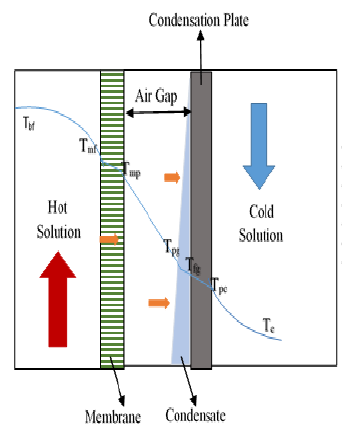
\includegraphics[width=0.72\linewidth]{tcc_images/chap03/Model-of-heat-and-mass-transfer-in-the-AGMD.png}\\[4pt]
      {\tiny Figura: Transporte de calor e massa na configuração AGMD. Fonte: Zheng (2017)}
    \end{column}
  \end{columns}
  \note{A destilação por membranas é um processo térmico onde a água salgada aquecida evapora na interface de uma membrana hidrofóbica e microporosa, o vapor atravessa os poros e condensa do lado frio. Não é filtração — a membrana não é molhada. As vantagens são do processo MD em geral. [~1 min]}
\end{slide}
%========================================================================

\begin{slide}{Fundamentos de Aprendizado de Máquinas}
  \footnotesize
  \vspace{-0.15cm}
  \centering
  \scriptsize
  \begin{tabular}{p{0.17\linewidth} p{0.38\linewidth} p{0.38\linewidth}}
      \toprule
      \textbf{Conceito} & \textbf{Definição} & \textbf{Propósito na Regressão} \\
      \midrule
      \textbf{Métricas}
      & RMSE (raiz do erro quadrático médio), R²
      & RMSE: magnitude do erro na mesma unidade; R²: proporção da variância explicada
      \\
      \midrule
      \textbf{Divisão dos dados}
      & Hold-out (80/20): separar treino, validação e teste
      & Evitar contaminação entre ajuste e avaliação \\
      \midrule
      \textbf{Busca de Hiperparâmetros}
      & Grid Search / Randomized Search sobre espaço de configurações
      & Encontrar a combinação de parâmetros que minimiza o erro de validação \\
      \midrule
      \textbf{Validação Cruzada}
      & Repetir a divisão em partições (K-fold) sem vazamento treino/validação
      & Estimar estabilidade do erro entre partições distintas \\
      \midrule
      \textbf{Validação por Grupos}
      & GroupKFold: mantém dados do mesmo \textbf{grupo} na mesma partição (diferente do K-fold tradicional, que mistura grupos)
      & Avaliar capacidade de extrapolação para grupos não vistos no treino \\
      \midrule
      \textbf{Pré-processamento}
      & Z-score (padronização para média zero e variância unitária)
      & Colocar variáveis em escala comparável, evitando que magnitudes distintas dominem o ajuste \\
      \midrule
      \textbf{Correlação}
      & \textbf{Pearson} ($r$): relação \textit{linear}. \textbf{Spearman} ($\rho$): relação \textit{monotônica}
      & Identificar relações lineares ou monotônicas entre entradas e saídas \\
      \bottomrule
    \end{tabular}
  \note{Campo: regressão supervisionada — prever saídas contínuas (fluxo, temperaturas) a partir de entradas operacionais. 1) Métricas, como medir. 2) Divisão: como separar treino e teste (80/20). 3) Busca de HP: otimização da configuração. 4) Validação cruzada: repetição da divisão para estimar estabilidade. 5) Validação por grupos: grupos inteiros ficam na mesma partição (diferente do K-fold tradicional), avaliando extrapolação. 6) Pré-processamento. 7) Correlação Pearson/Spearman: relações lineares e monotônicas. [~1,5 min]}
\end{slide}

%========================================================================

\begin{slide}{Famílias de Modelos I — Regressão Linear e Regularizadas}
  \centering
  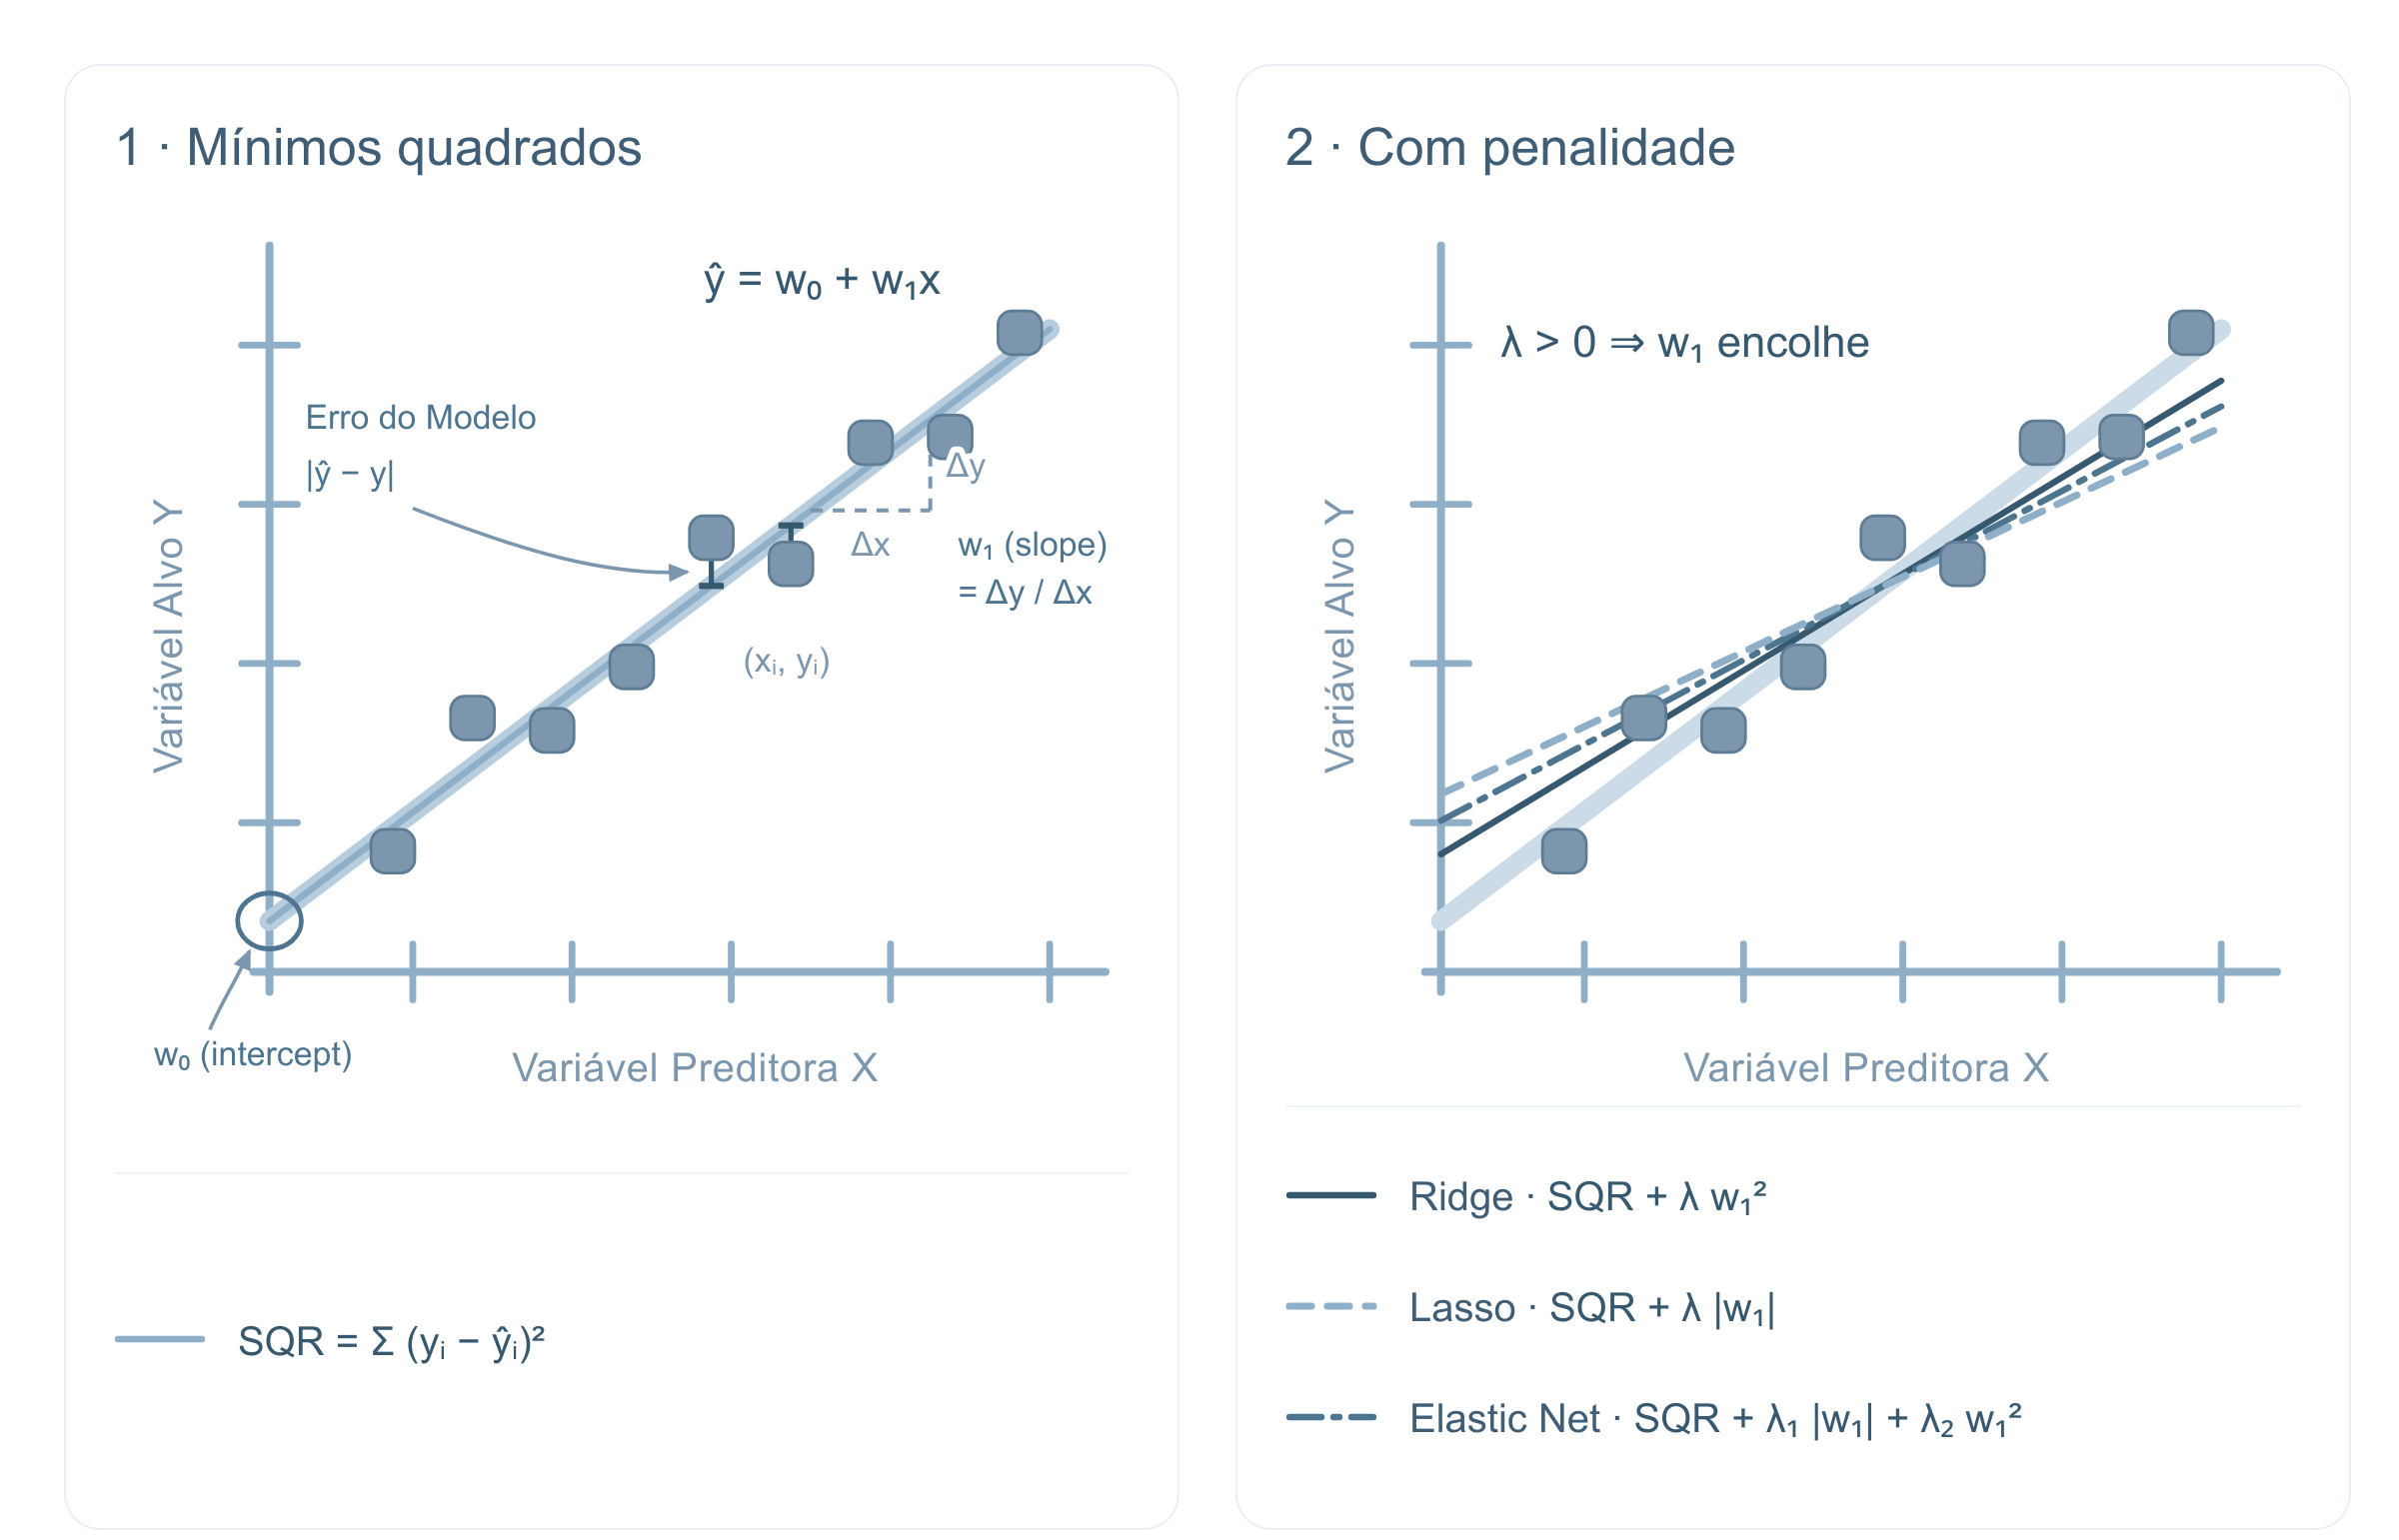
\includegraphics[width=0.62\textwidth]{tcc_images/chap02a/regressao.png}
  \vfill
  {\scriptsize Fonte: Autor}
  \note{Lineares: OLS sem regularização, Ridge penaliza L2 (encolhe coeficientes), Lasso penaliza L1 (zera coeficientes — seleção de variáveis), ElasticNet combina ambos. [~45s]}
\end{slide}
%========================================================================
\begin{slide}{Famílias de Modelos II — Árvores de Decisão}
  \centering
  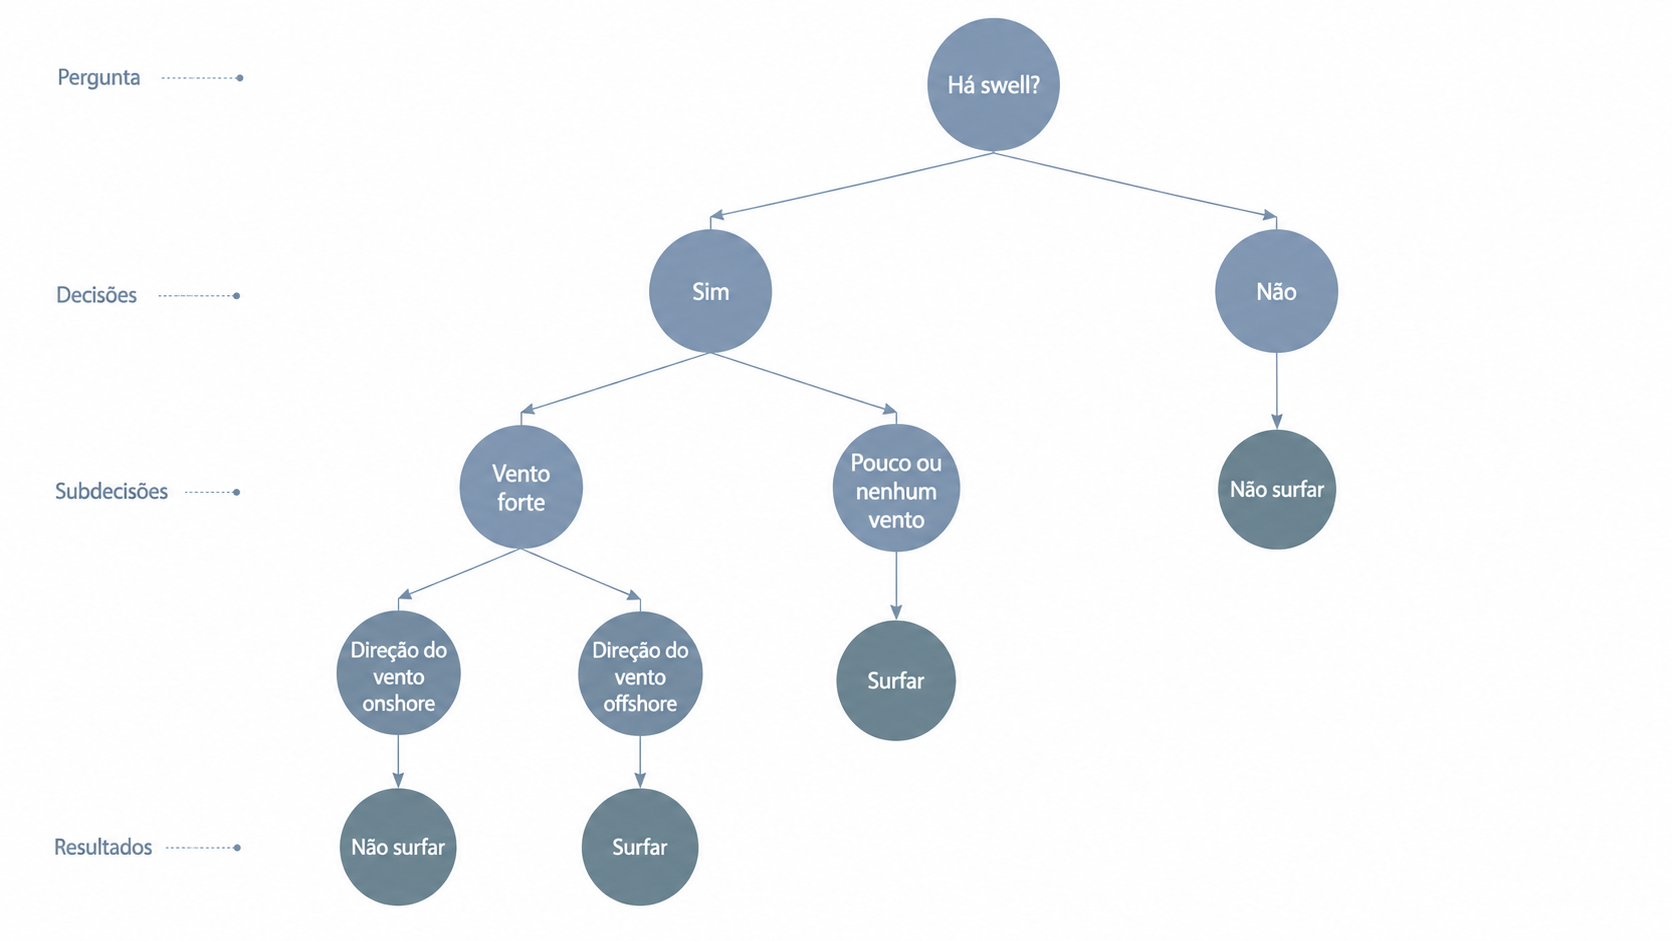
\includegraphics[width=0.68\textwidth]{tcc_images/chap02a/arvores.png}
  \vfill
  {\scriptsize Fonte: Autor}
  \note{Árvores: DT overfitta, RF reduz variância com bagging, GB corrige resíduos sequencialmente. [~45s]}
\end{slide}
%========================================================================
\begin{slide}{Famílias de Modelos III — Redes Neurais}
  \centering
  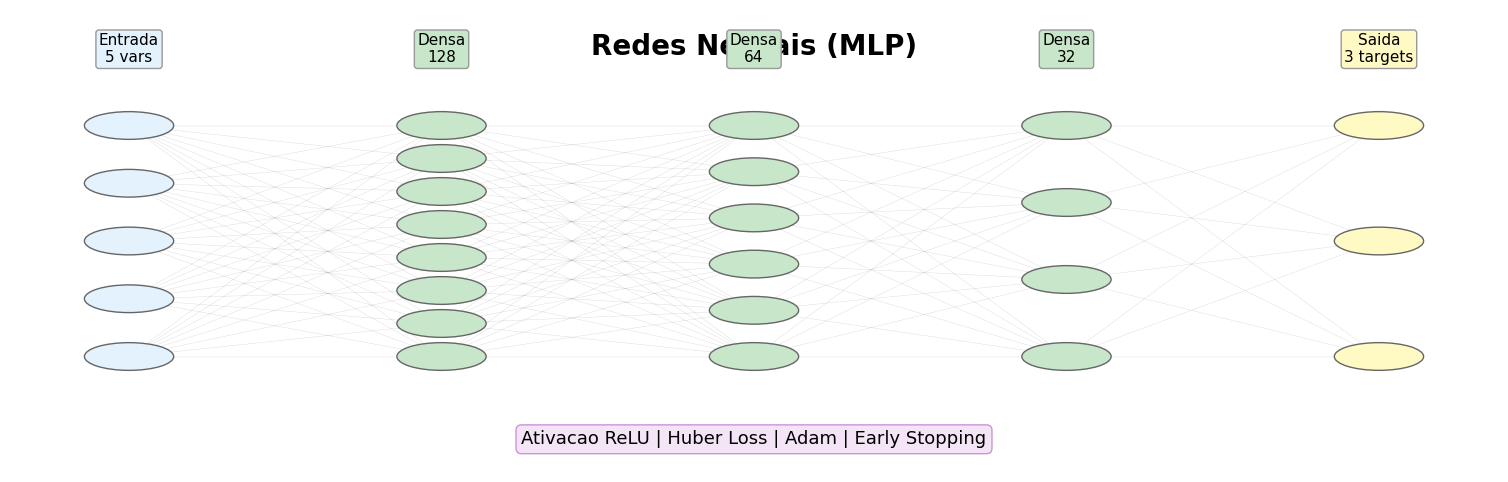
\includegraphics[width=0.78\textwidth]{tcc_images/chap02a/redes_neurais.png}
  \vfill
  {\scriptsize Fonte: Autor}
  \note{MLP: camadas totalmente conectadas, com backpropagation para ajuste dos coeficientes. Hiperparâmetros: camadas, neurônios, ativação, lr, L2. [~45s]}
\end{slide}
%========================================================================
\begin{slide}{Famílias de Modelos IV — Arquiteturas Híbridas}
  \centering
  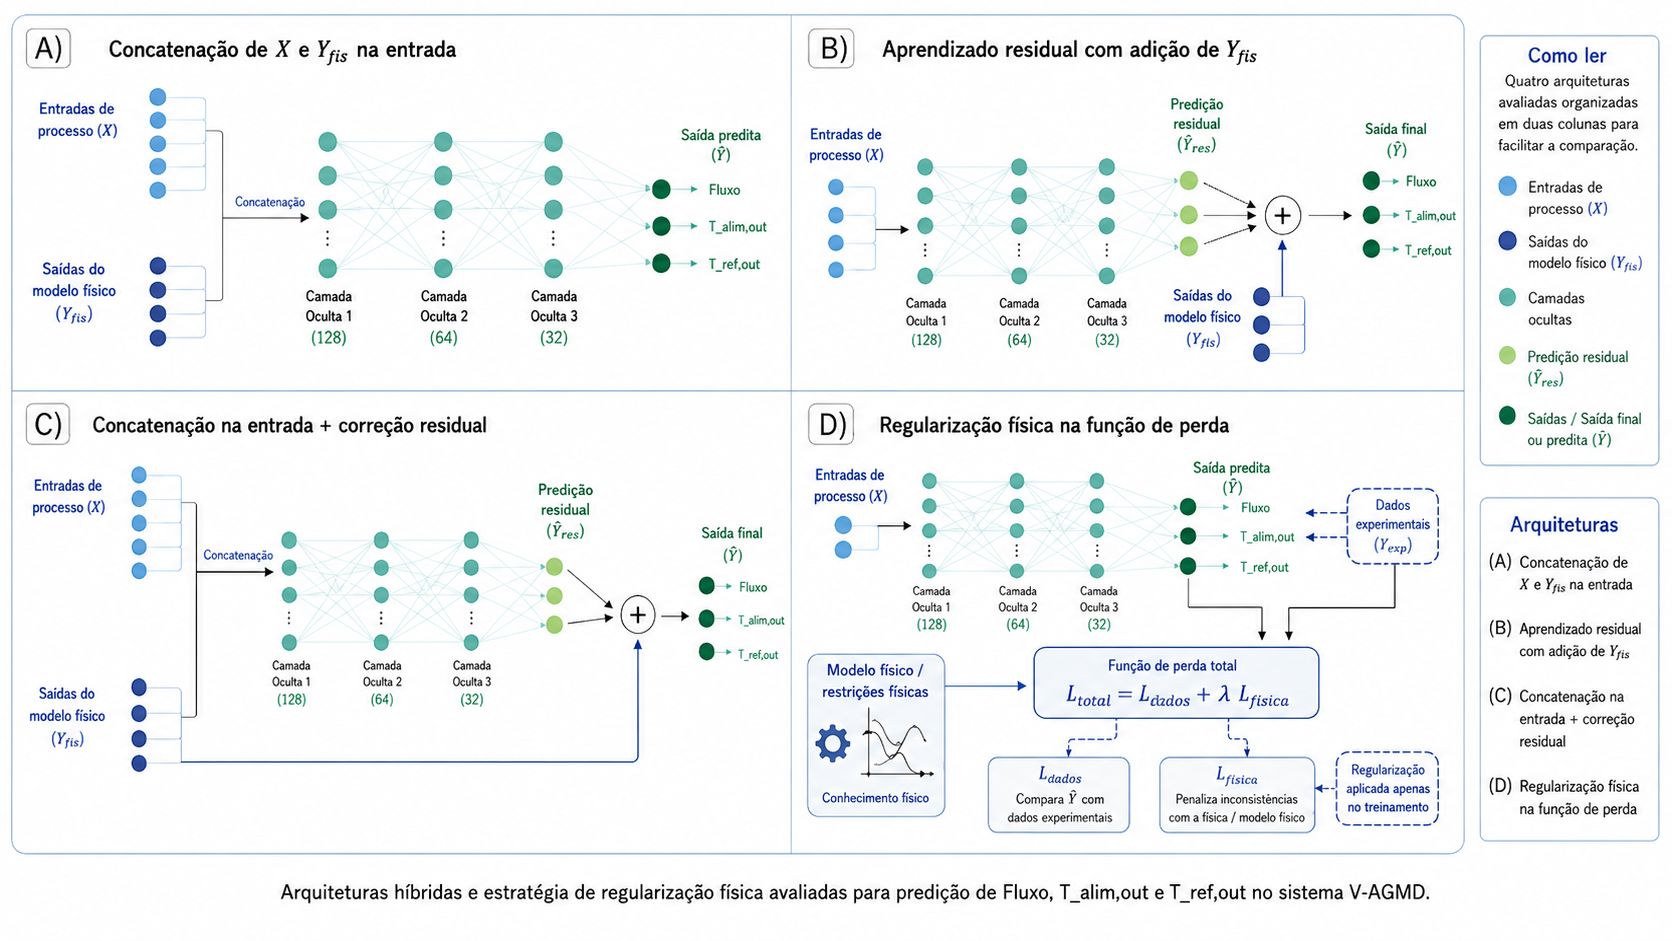
\includegraphics[width=0.78\textwidth]{tcc_images/chap02a/hibridos-slides.png}
  \vfill
  {\scriptsize Fonte: Autor}
  \note{Híbridos: quatro arquiteturas que incorporam o modelo físico 0D. [~30s]}
\end{slide}
%========================================================================



    	\section{Metodologia Proposta}

\begin{slide}{Visão Geral dos Procedimentos}
  \centering
  \resizebox{0.9\textwidth}{!}{%
  \begin{tikzpicture}[
      every node/.style={font=\footnotesize},
      stage/.style={rectangle, rounded corners, draw=poliBlue, thick, align=center,
                    minimum width=2cm, minimum height=0.65cm, fill=blue!6},
      arrow/.style={->, thick, >=stealth},
      darrow/.style={->, thick, >=stealth, dashed},
      detail/.style={rectangle, rounded corners, draw=black!40, thick, align=center, font=\tiny, minimum width=2.2cm, minimum height=0.4cm, fill=gray!6},
    ]
    % Row 1
    \node[stage] (dados)      {Dados\\Experimentais};
    \node[stage, right=0.35cm of dados] (prep)  {Preparação\\dos Dados};
    \node[detail, below=0.1cm of prep, font=\tiny, draw=black!40, thick, minimum width=1.8cm, minimum height=0.35cm] {Z-score};
    \node[stage, right=0.35cm of prep] (eda)    {Análise\\Exploratória};
    \node[stage, right=0.35cm of eda] (sel) {Validação e\\Seleção};
    \draw[arrow] (dados) -- (prep);
    \draw[arrow] (prep) -- (eda);
    \draw[arrow] (eda) -- (sel);


    % Row 2
    \node[stage, below=0.9cm of sel] (fisico) {Modelo\\Físico 0D};
    \node[stage, right=0.35cm of fisico] (s0)    {Stage 0\\Clássicos};
    \node[stage, right=0.35cm of s0] (s1)    {Stage 1\\Redes Neurais};
    \node[stage, right=0.35cm of s1] (s2)    {Stage 2\\Híbridos};
    \draw[arrow] (fisico) -- (s0);
    \draw[arrow] (s0) -- (s1);
    \draw[arrow] (s1) -- (s2);
    % Connection Row1 -> Row2
    \draw[darrow] (sel.south) -- ++(0,-0.1) -| (fisico.north);

    % Row 3
    \node[stage, below=0.9cm of s2] (final) {Selecionado\\vs 0D};
    \draw[arrow] (s2) -- (final);

    % Connection Row2 -> Row3
    \draw[darrow] (s2.south) -- (final.north);
  \end{tikzpicture}
  }
  \note{Visão geral dos procedimentos: dados, preparação, análise exploratória, modelo físico 0D, Stage 0 (clássicos), Stage 1 (redes neurais), Stage 2 (híbridos), seleção pelo critério 1-SE e comparação final. [~1,5 min]}
\end{slide}
\begin{slide}{Etapa 1: Dados Experimentais}
  \small
  \begin{columns}
    \begin{column}{.35\linewidth}
      \begin{Item}
        \item 174 pontos experimentais do sistema V-AGMD piloto (LabMEMS/COPPE) \cite{curcino2023,Lisboa2024}
        \item 3 regimes de salinidade: 10, 40 e 70 g/L de NaCl
        \item 5 entradas: T$_{in,alim}$, T$_{in,ref}$, vazão$_{ref}$, P$_{vac}$, C$_{NaCl}$
        \item 3 saídas: Fluxo de permeado, T$_{out,alim}$, T$_{out,ref}$
      \end{Item}
      \vfill
      {\scriptsize Fonte dos dados: \cite{curcino2023,Lisboa2024}}
    \end{column}
    \begin{column}{.65\linewidth}
      \centering
      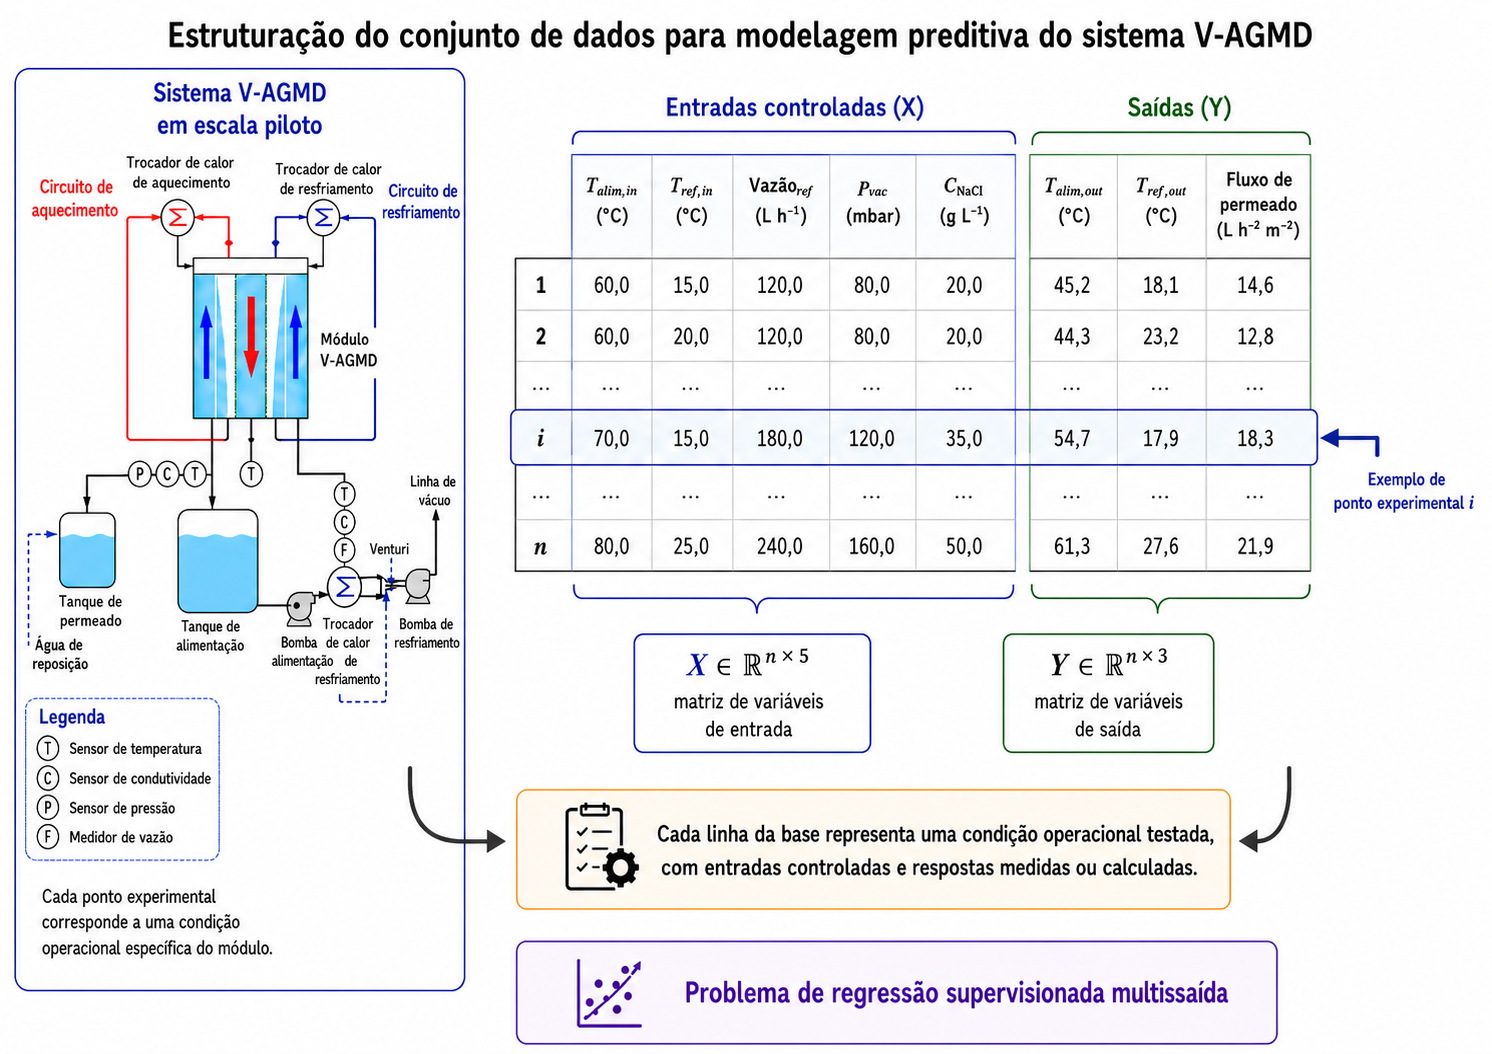
\includegraphics[width=\linewidth]{tcc_images/chap04/esquematizacao_regressao.png}
    \end{column}
  \end{columns}
  \note{O conjunto de dados tem 174 pontos experimentais obtidos em um sistema V-AGMD piloto, disponibilizado por Curcino et al. (2023) e Lisboa et al. (2024). Foram testados 3 regimes de salinidade: 10, 40 e 70 g/L. As 5 variáveis de entrada incluem temperaturas, vazão, pressão de vácuo e concentração salina. As 3 saídas são o fluxo de permeado e as duas temperaturas de saída. [~1 min]}
\end{slide}
\begin{slide}{Resumo — Decisões da Preparação dos Dados}
  \centering
  \small
  \begin{tabular}{lcp{7.5cm}}
    \rowcolor{poliBlue!20}
    \textbf{Etapa} & \textbf{Decisão} & \textbf{Justificativa} \\ \hline
    \rowcolor{gray!10}
    2.1 — Escalonamento & Z-score &
    Preserva a distribuição original dos dados; mede cada ponto em desvios-padrão, evitando compressão artificial na presença de valores extremos \\
    \rowcolor{white}
    2.2 — Validação & GroupKFold &
    Separa os folds por regime operacional, orientando a busca de hiperparâmetros para capacidade de \textbf{extrapolação} — diferente do KFold comum, que só avalia interpolação \\
  \end{tabular}
  \note{Slide de consolidação: resume as decisões de preparação dos dados e suas justificativas. [~1 min]}
\end{slide}
%========================================================================

\begin{slide}{Busca de Hiperparâmetros}
  \centering
  \small
  \begin{Item}
    \item Para cada família de modelos e cada \textbf{variável de saída} (target), foi realizado um ajuste independente de hiperparâmetros
    \item \textbf{Redes Neurais (MLP/Keras)}: \textbf{Random Search} (amostragem aleatória da grade) — maior espaço de busca (arquitetura, taxa de aprendizado, regularização)
    \item \textbf{Demais famílias} (lineares, árvores, híbridos): \textbf{busca exaustiva} (GridSearchCV) — espaço menor de hiperparâmetros
    \item Híbridos residuais: busca restrita (apenas regularização L2) para isolar o efeito da incorporação da física
  \end{Item}
  \vfill
  {\scriptsize \textbf{Legenda de cores:} \textcolor{blue!70!black}{azul} = modelos lineares \; \textcolor{green!70!black}{verde} = árvores de decisão \; \textcolor{orange!70!black}{laranja} = redes neurais \; \textcolor{red!70!black}{vermelho} = modelos híbridos (física + dados)}
  \note{A busca de hiperparâmetros foi feita por família e por target. Redes neurais usaram Random Search (espaço maior); as demais famílias usaram busca exaustiva. Híbridos residuais tiveram busca restrita (só L2). [~1,5 min]}
\end{slide}
%========================================================================

\begin{frame}
  \centering
  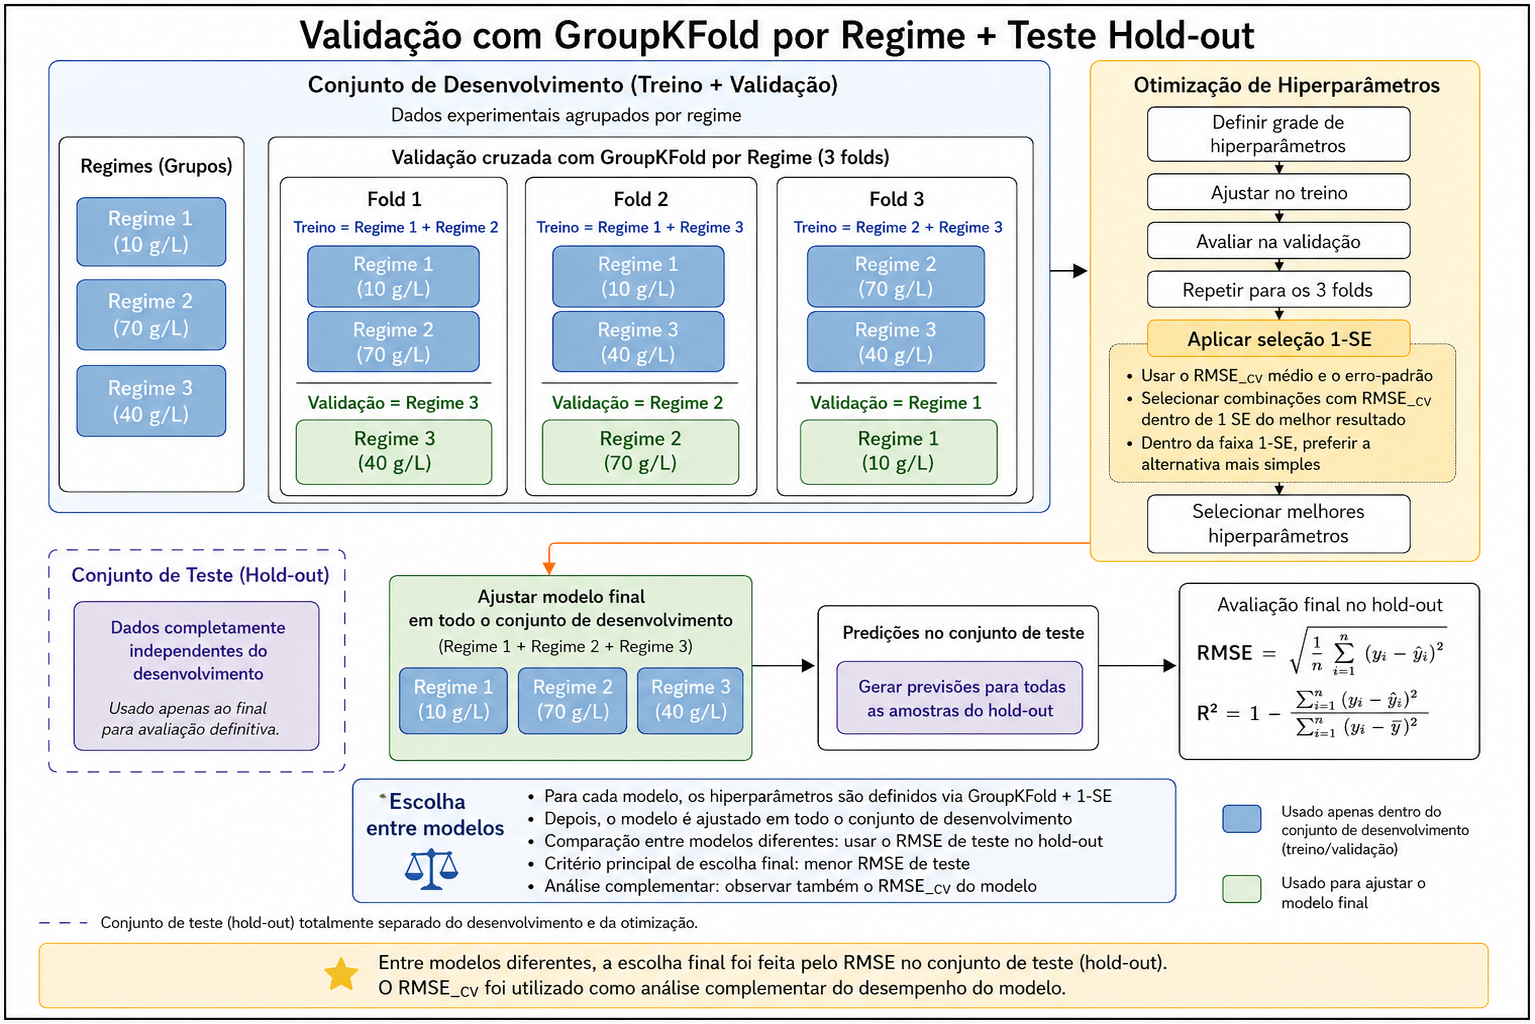
\includegraphics[width=0.75\linewidth]{tcc_images/chap04/criterio_selecao_esquema.png}
  \vfill
  {\scriptsize Fonte: Autor}
  \note{O fluxo completo: GroupKFold por regimes $\rightarrow$ RMSE$_{CV}$ m�dio com erro padr�o $\rightarrow$ regra 1-SE $\rightarrow$ sele��o do modelo mais simples dentro de 1 erro padr�o do melhor. [~1 min]}
\end{frame}


    	\section{Resultados}

\begin{slide}{Análise Exploratória}
  \footnotesize
  \begin{columns}
    \begin{column}{.35\linewidth}
      \begin{Item}[0.15]
        \item Dispersão: T$_{out}$ correlacionada com entradas térmicas; fluxo com múltiplas variáveis
        \item Pearson: T$_{out}$ têm correlações lineares fortes ($|r|>0,9$); fluxo moderado ($|r|\approx0,7$)
        \item Spearman: valores próximos aos de Pearson $\rightarrow$ relações dominantes são aproximadamente lineares (monotônicas e lineares)
        \item Complexidade do fluxo $\rightarrow$ justifica modelagem multivariada
      \end{Item}
    \end{column}
    \begin{column}{.65\linewidth}
      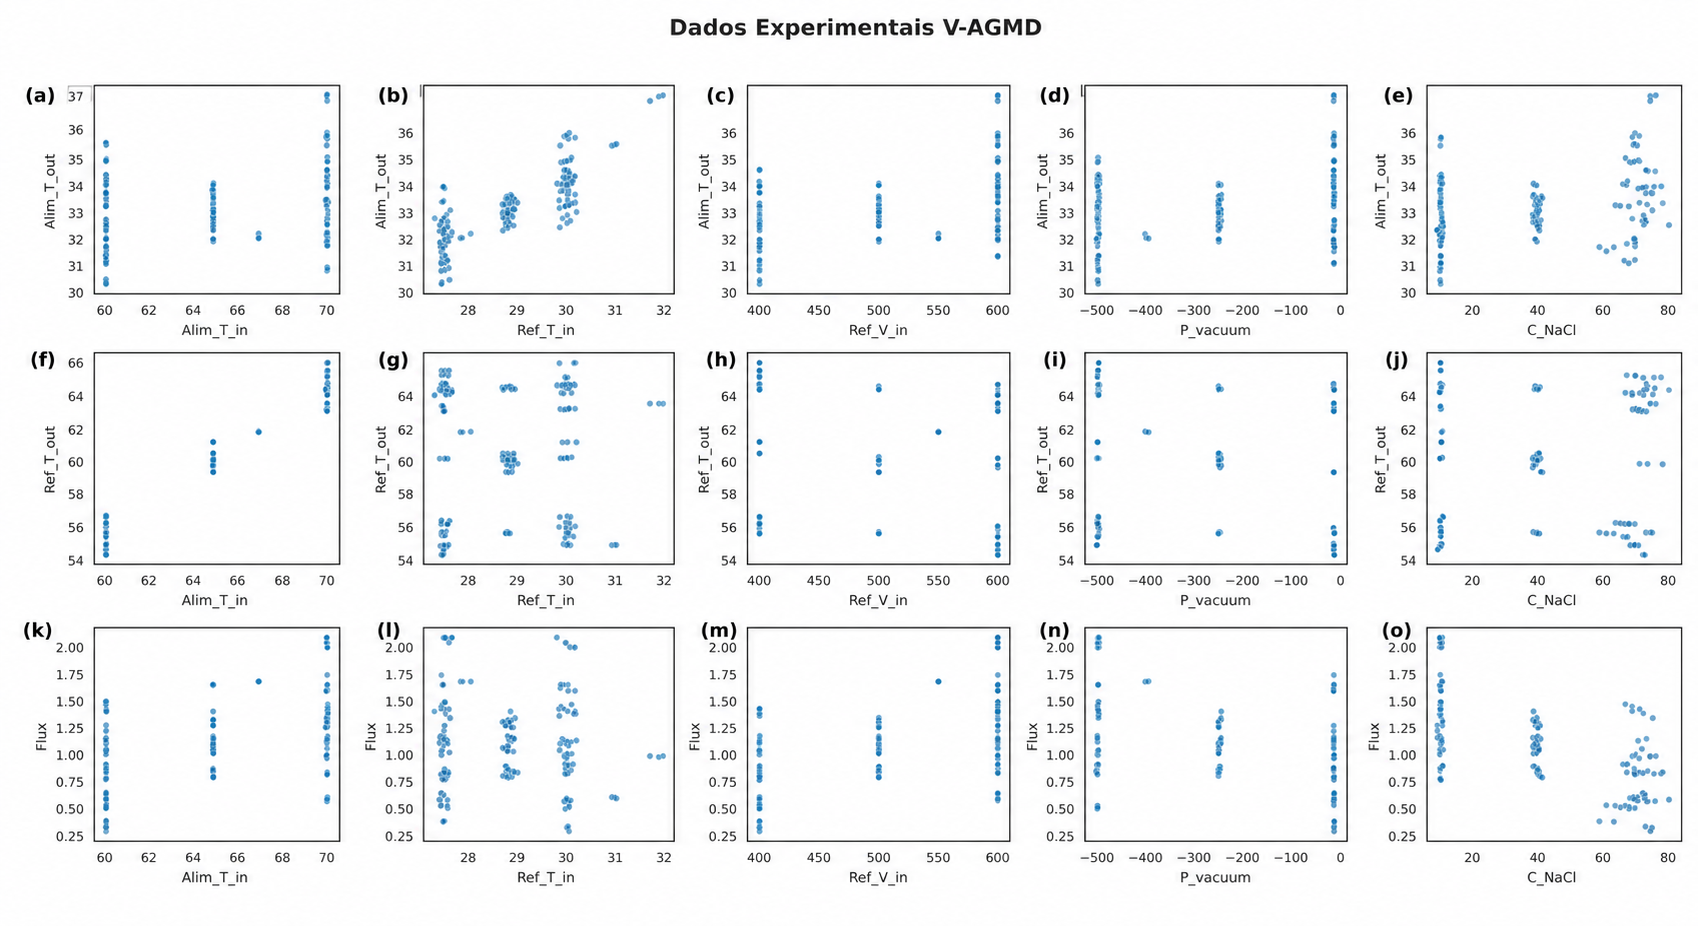
\includegraphics[width=\linewidth]{tcc_images/chap06/scatter_vagmd_exp_only.png}
    \end{column}
  \end{columns}
  \note{Análise exploratória: temperaturas de saída têm forte correlação linear (Pearson e Spearman próximos), fluxo é mais complexo. [~1 min]}
\end{slide}
%========================================================================

\begin{slide}{Modelo Físico 0D — Referência}
  \centering
  O modelo 0D de \cite{Lisboa2024} serve como referência fenomenológica para as arquiteturas híbridas. Não é um modelo desenvolvido neste trabalho.
  \vfill
  \begin{columns}
    \begin{column}{.33\linewidth}
      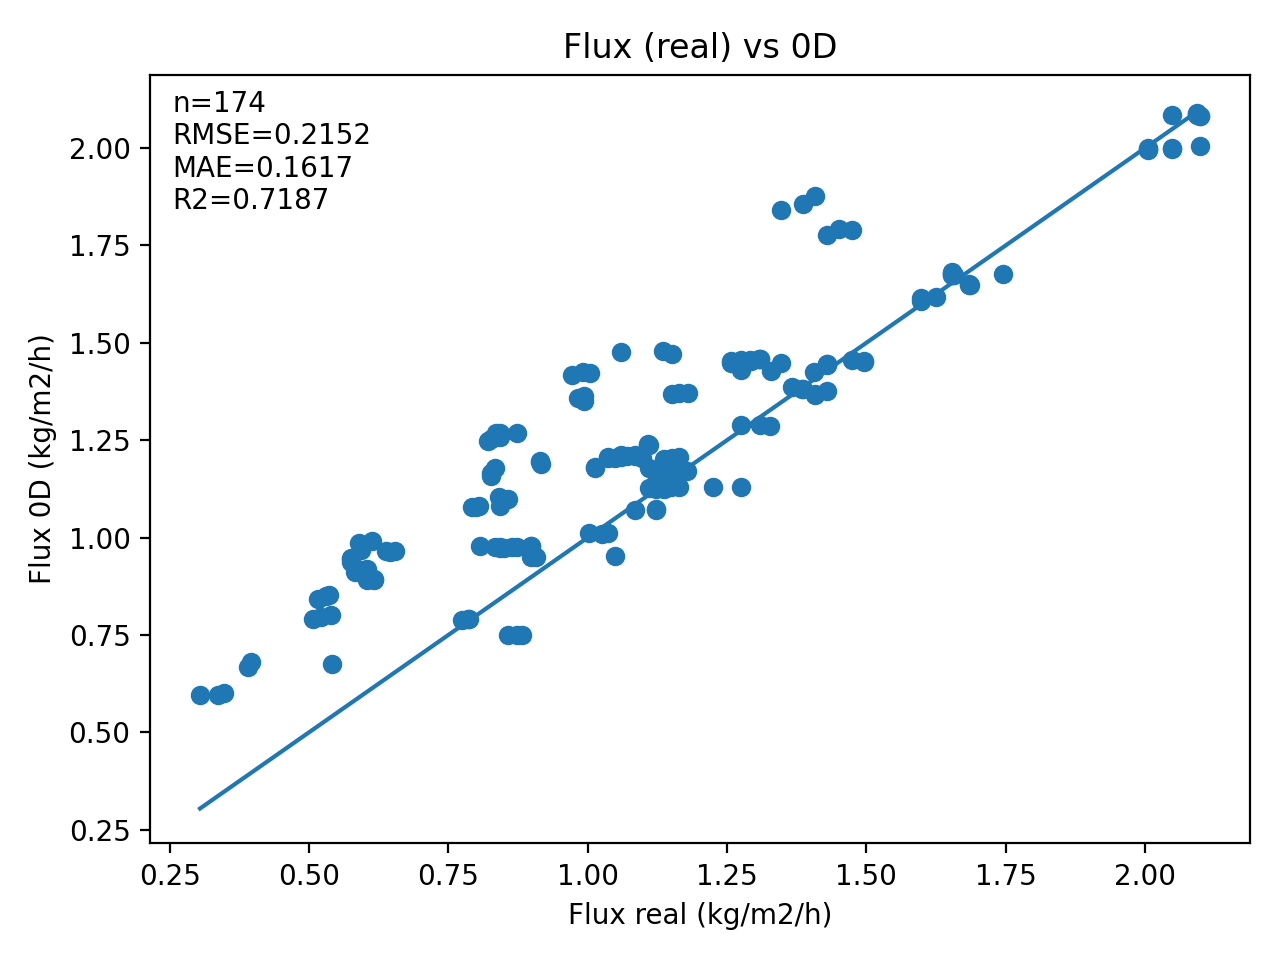
\includegraphics[width=\linewidth]{tcc_images/chap06/flux_real_vs_0d.png}
    \end{column}
    \begin{column}{.33\linewidth}
      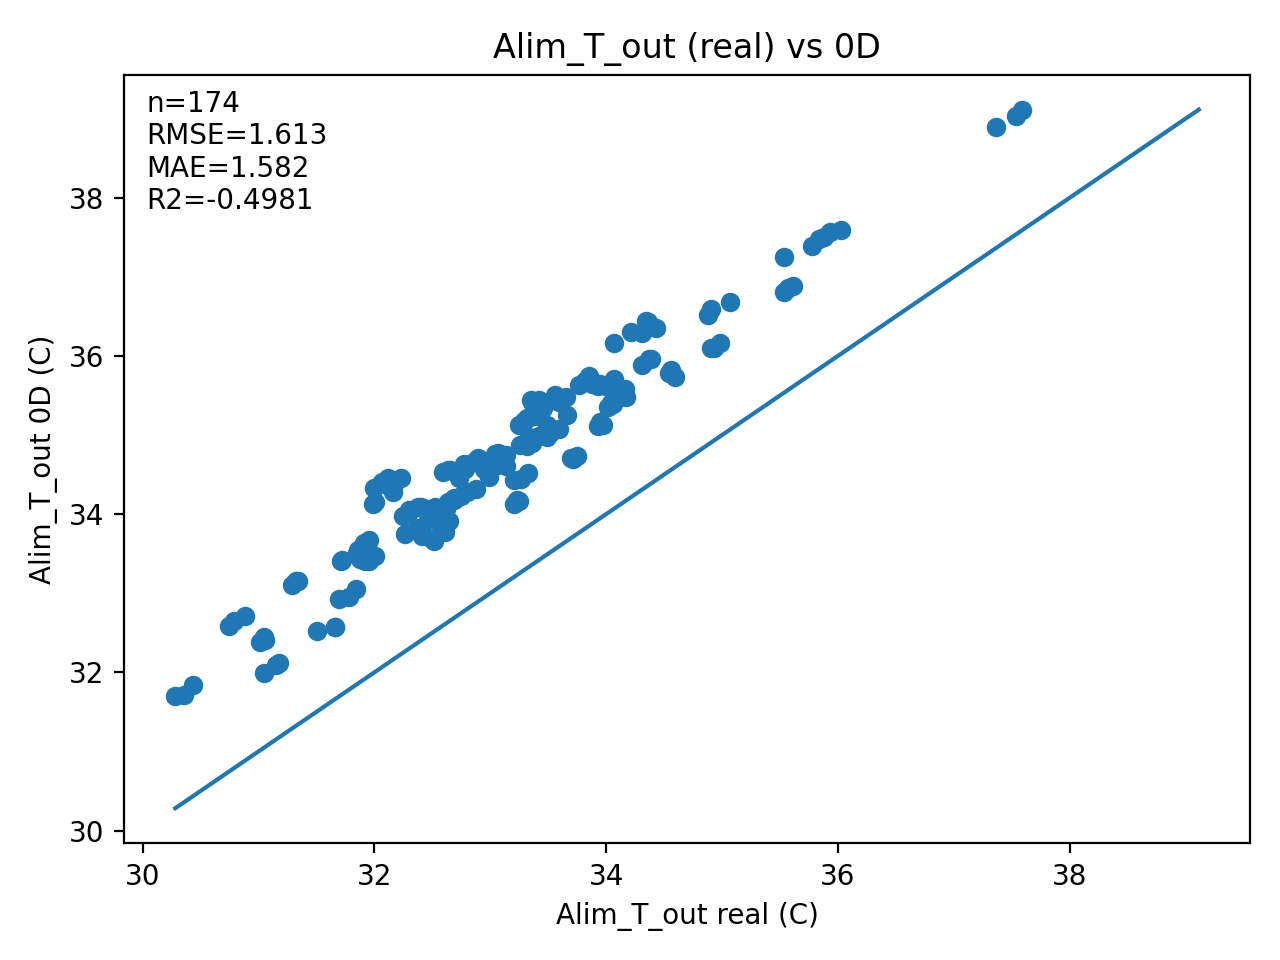
\includegraphics[width=\linewidth]{tcc_images/chap06/alim_T_out_real_vs_0d.png}
    \end{column}
    \begin{column}{.33\linewidth}
      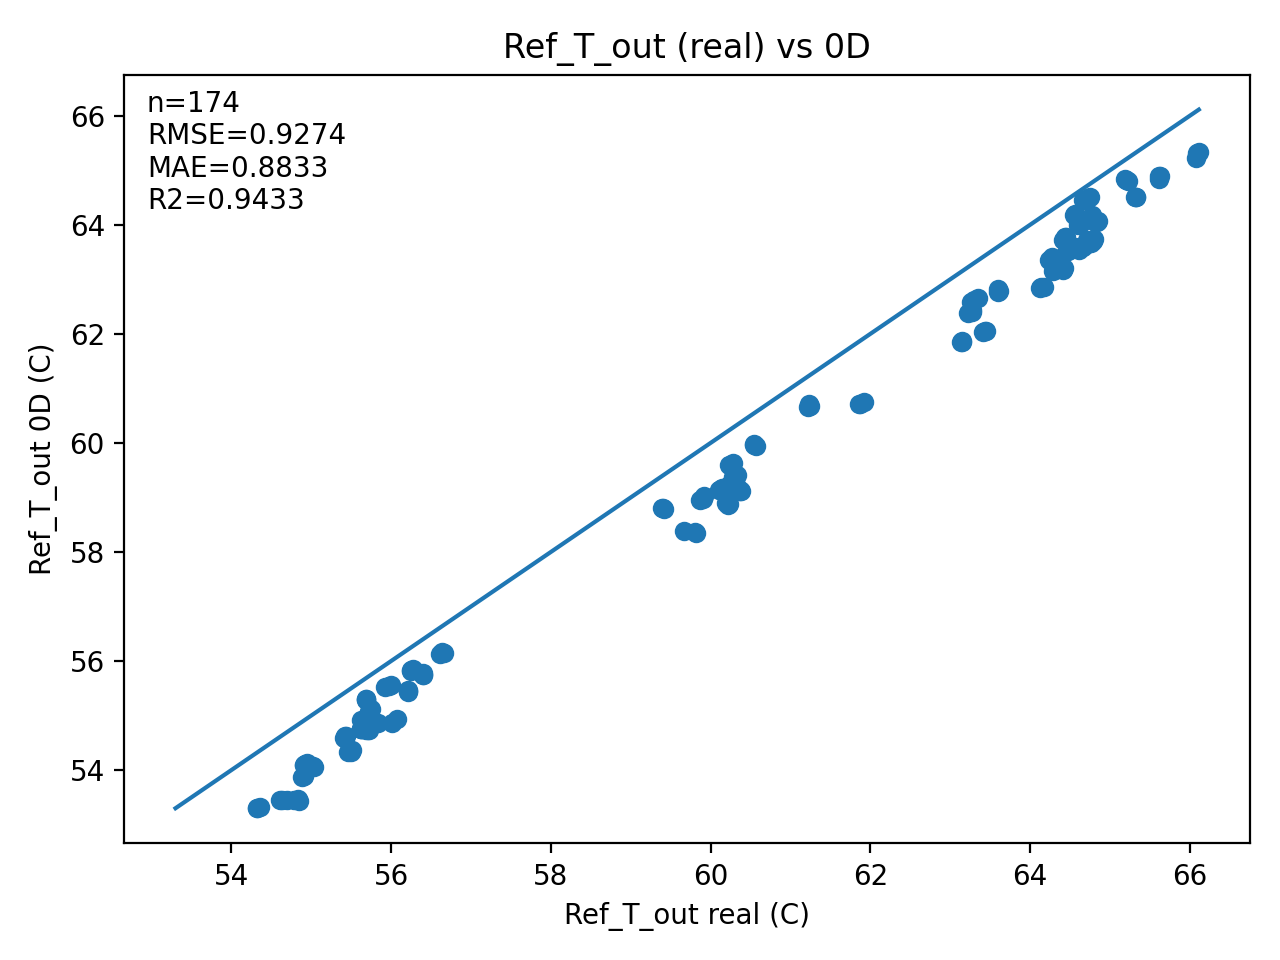
\includegraphics[width=\linewidth]{tcc_images/chap06/ref_T_out_real_vs_0d.png}
    \end{column}
  \end{columns}
  \vfill
  {\scriptsize Predição do modelo 0D \textit{vs} experimental para cada variável de saída. Modelo 0D: \cite{Lisboa2024}}
  \note{O modelo 0D de Lisboa et al. (2024) é a referência física — não é um modelo desenvolvido neste trabalho. As arquiteturas híbridas aprendem a corrigir sistematicamente suas predições a partir dos dados experimentais. [~30s]}
\end{slide}
%========================================================================

% Tabela detalhada removida a pedido da orientadora (S30-S34): manter apenas a tabela consolidada
% \begin{slide}{Stage 0 — Modelos Lineares}
%   ... (conteúdo movido para o material suplementar)
% \end{slide}

\begin{slide}{Stage 0 — Modelos Lineares e Árvores}
  \centering
  \small
  \textbf{Modelos lineares} (OLS, Ridge, Lasso, ElasticNet): desempenho similar entre si; regularização não trouxe ganho significativo sobre OLS.
  \vfill
  \textbf{Árvores de decisão} (DT, RF, GB): DT e RF overfitam nos regimes de treino (CV alto); GB generaliza melhor, mas ainda inferior aos lineares.
  \vfill
  {\scriptsize Detalhes das tabelas de Stage 0 no material suplementar.}
  \note{Stage 0: lineares — OLS, Ridge, Lasso, ElasticNet têm desempenho similar. Árvores — DT e RF overfitam; GB generaliza melhor mas inferior aos lineares. [~1 min]}
\end{slide}
%========================================================================

% Tabela detalhada removida a pedido da orientadora (S30-S34): manter apenas a tabela consolidada
% \begin{slide}{Stage 0 — Árvores de Decisão}
%   ... (conteúdo movido para o material suplementar)
% \end{slide}
%========================================================================

\begin{slide}{Stage 1 — Redes Neurais}
  \centering
  \scriptsize
  \begin{tabular}{llcccccc}
    \toprule
    \textbf{Arquitetura} & \textbf{Alvo} & \multicolumn{3}{c}{\textbf{CV RMSE}} & \multicolumn{3}{c}{\textbf{Test RMSE}} \\
    \cmidrule(lr){3-5} \cmidrule(lr){6-8}
    & & T$_{alim}$ & T$_{ref}$ & Flux & T$_{alim}$ & T$_{ref}$ & Flux \\
    \midrule
    (128,64), tanh, lr=0,001, l2=0,001 & Alim & 0,260 & \textbf{0,445} & 0,115 & 0,215 & \cellcolor{orange!10}\textbf{0,309} & 0,073 \\
    (128,64), tanh, lr=0,001, l2=0,001 & Ref & 0,267 & 0,459 & 0,116 & 0,227 & 0,318 & 0,073 \\
    (128,64,32), relu, lr=0,003, l2=0,0 & Flux & \textbf{0,222} & 0,554 & \textbf{0,081} & \cellcolor{blue!10}\textbf{0,178} & 0,369 & \cellcolor{green!10}\textbf{0,066} \\
    \bottomrule
  \end{tabular}
  \note{Três baselines de redes neurais. A otimizada para Flux tem arquitetura maior (128,64,32) mas L2=0. [~1 min]}
\end{slide}
%========================================================================

\begin{slide}{Stage 2 — Modelos Híbridos}
  \centering
  \scriptsize
  \begin{tabular}{llcccccc}
    \toprule
    \textbf{Modelo} & \textbf{Alvo} & \multicolumn{3}{c}{\textbf{CV RMSE}} & \multicolumn{3}{c}{\textbf{Test RMSE}} \\
    \cmidrule(lr){3-5} \cmidrule(lr){6-8}
    & & T$_{alim}$ & T$_{ref}$ & Flux & T$_{alim}$ & T$_{ref}$ & Flux \\
    \midrule
    \textbf{PhyResidual} & \textbf{Alim} & 0,275 & \textbf{0,301} & \textbf{0,060} & 0,225 & 0,222 & 0,057 \\
    \textbf{PhyResidual} & \textbf{Ref} & 0,274 & 0,305 & 0,061 & 0,224 & 0,231 & 0,058 \\
    \rowcolor{green!6}
    \textbf{PhyResidual} & \textbf{Flux} & \textbf{0,236} & 0,346 & 0,072 & \cellcolor{blue!10}\textbf{0,183} & \cellcolor{orange!10}\textbf{0,214} & \cellcolor{green!10}\textbf{0,054} \\
    PhyHybrid & Alim & 0,273 & 0,306 & 0,061 & 0,224 & 0,231 & 0,058 \\
    PhyHybrid & Ref & 0,275 & 0,302 & 0,061 & 0,225 & 0,230 & 0,058 \\
    PhyHybrid & Flux & 0,284 & 0,399 & 0,075 & 0,222 & 0,239 & 0,055 \\
    PhyInput & Alim & 0,273 & 0,325 & 0,098 & 0,213 & 0,250 & 0,064 \\
    PhyInput & Ref & 0,275 & 0,432 & 0,106 & 0,216 & 0,269 & 0,066 \\
    PhyInput & Flux & 0,260 & 0,625 & 0,104 & 0,213 & 0,426 & 0,063 \\
    \midrule
    PhyLoss ($\omega{=}0{,}0$) & Alim & 0,180 & 0,348 & 0,067 & 0,188 & 0,350 & 0,068 \\
    PhyLoss ($\omega{=}0{,}7$) & Ref  & 0,310 & 0,276 & 0,192 & 0,340 & 0,286 & 0,220 \\
    PhyLoss ($\omega{=}0{,}0$) & Flux & 0,203 & 0,422 & 0,066 & 0,226 & 0,438 & 0,069 \\
    \bottomrule
  \end{tabular}
  \note{PhyResidual (base Flux) teve o menor Test RMSE nos três alvos entre os híbridos. Para T\_ref, diferença sobre Ridge é marginal (2,3\%); Ridge tem melhor CV (extrapolação). [~2 min]}
\end{slide}
%========================================================================

\begin{slide}{Comparação Final — Consolidado por Variável de Saída}
  \centering
  \footnotesize
    \begin{tabular}{lclcccc}
    \toprule
    \textbf{Variável de saída} & \textbf{Estágio} & \textbf{Modelo} & \textbf{Test RMSE} & \textbf{CV RMSE} & \textbf{Test R$^2$} \\
    \midrule
    \textbf{T$_{alim,out}$} & Stage 0 & OLS & 0,231 & \textbf{0,196} & 0,965 \\
    \textbf{T$_{alim,out}$} & Stage 1 & Baseline Flux & \textbf{0,178} & 0,081 & 0,981 \\
    \textbf{T$_{alim,out}$} & Stage 2 & PhyResidual (Flux) & 0,183 & 0,275 & 0,981 \\
    \midrule
    \textbf{T$_{ref,out}$} & Stage 0 & Ridge (Ref) & 0,219 & \cellcolor{yellow!15}\textbf{0,244} & 0,996 \\
    \textbf{T$_{ref,out}$} & Stage 1 & Baseline Alim & 0,309 & 0,445 & 0,989 \\
    \textbf{T$_{ref,out}$} & Stage 2 & PhyResidual (Flux) & \textbf{0,214} & 0,346 & \textbf{0,996} \\
    \midrule
    \textbf{Flux} & Stage 0 & Lasso (Flux) & 0,075 & 0,082 & 0,951 \\
    \textbf{Flux} & Stage 1 & Baseline Flux & 0,066 & 0,081 & 0,972 \\
    \textbf{Flux} & Stage 2 & PhyResidual (Flux) & \textbf{0,054} & \textbf{0,072} & \textbf{0,979} \\
    \midrule
    \rowcolor{gray!6}
    \textbf{Flux} & \multirow{3}{*}{\textbf{Modelo 0D}} & --- & 0,206 & --- & 0,631 \\
    \rowcolor{gray!6}
    \textbf{T$_{alim,out}$} & & --- & 1,549 & --- & $-$0,404 \\
    \rowcolor{gray!6}
    \textbf{T$_{ref,out}$} & & --- & 0,851 & --- & 0,948 \\
    \bottomrule
  \end{tabular}
  \note{Test RMSE em negrito = menor erro por variável; CV RMSE em negrito = melhor generalização. O Flux foi a única saída onde o menor Test RMSE e o menor CV RMSE pertencem ao mesmo modelo. [~2 min]}
\end{slide}
%========================================================================

\begin{slide}{Predição vs Experimental — Modelos Selecionados}
  \centering
  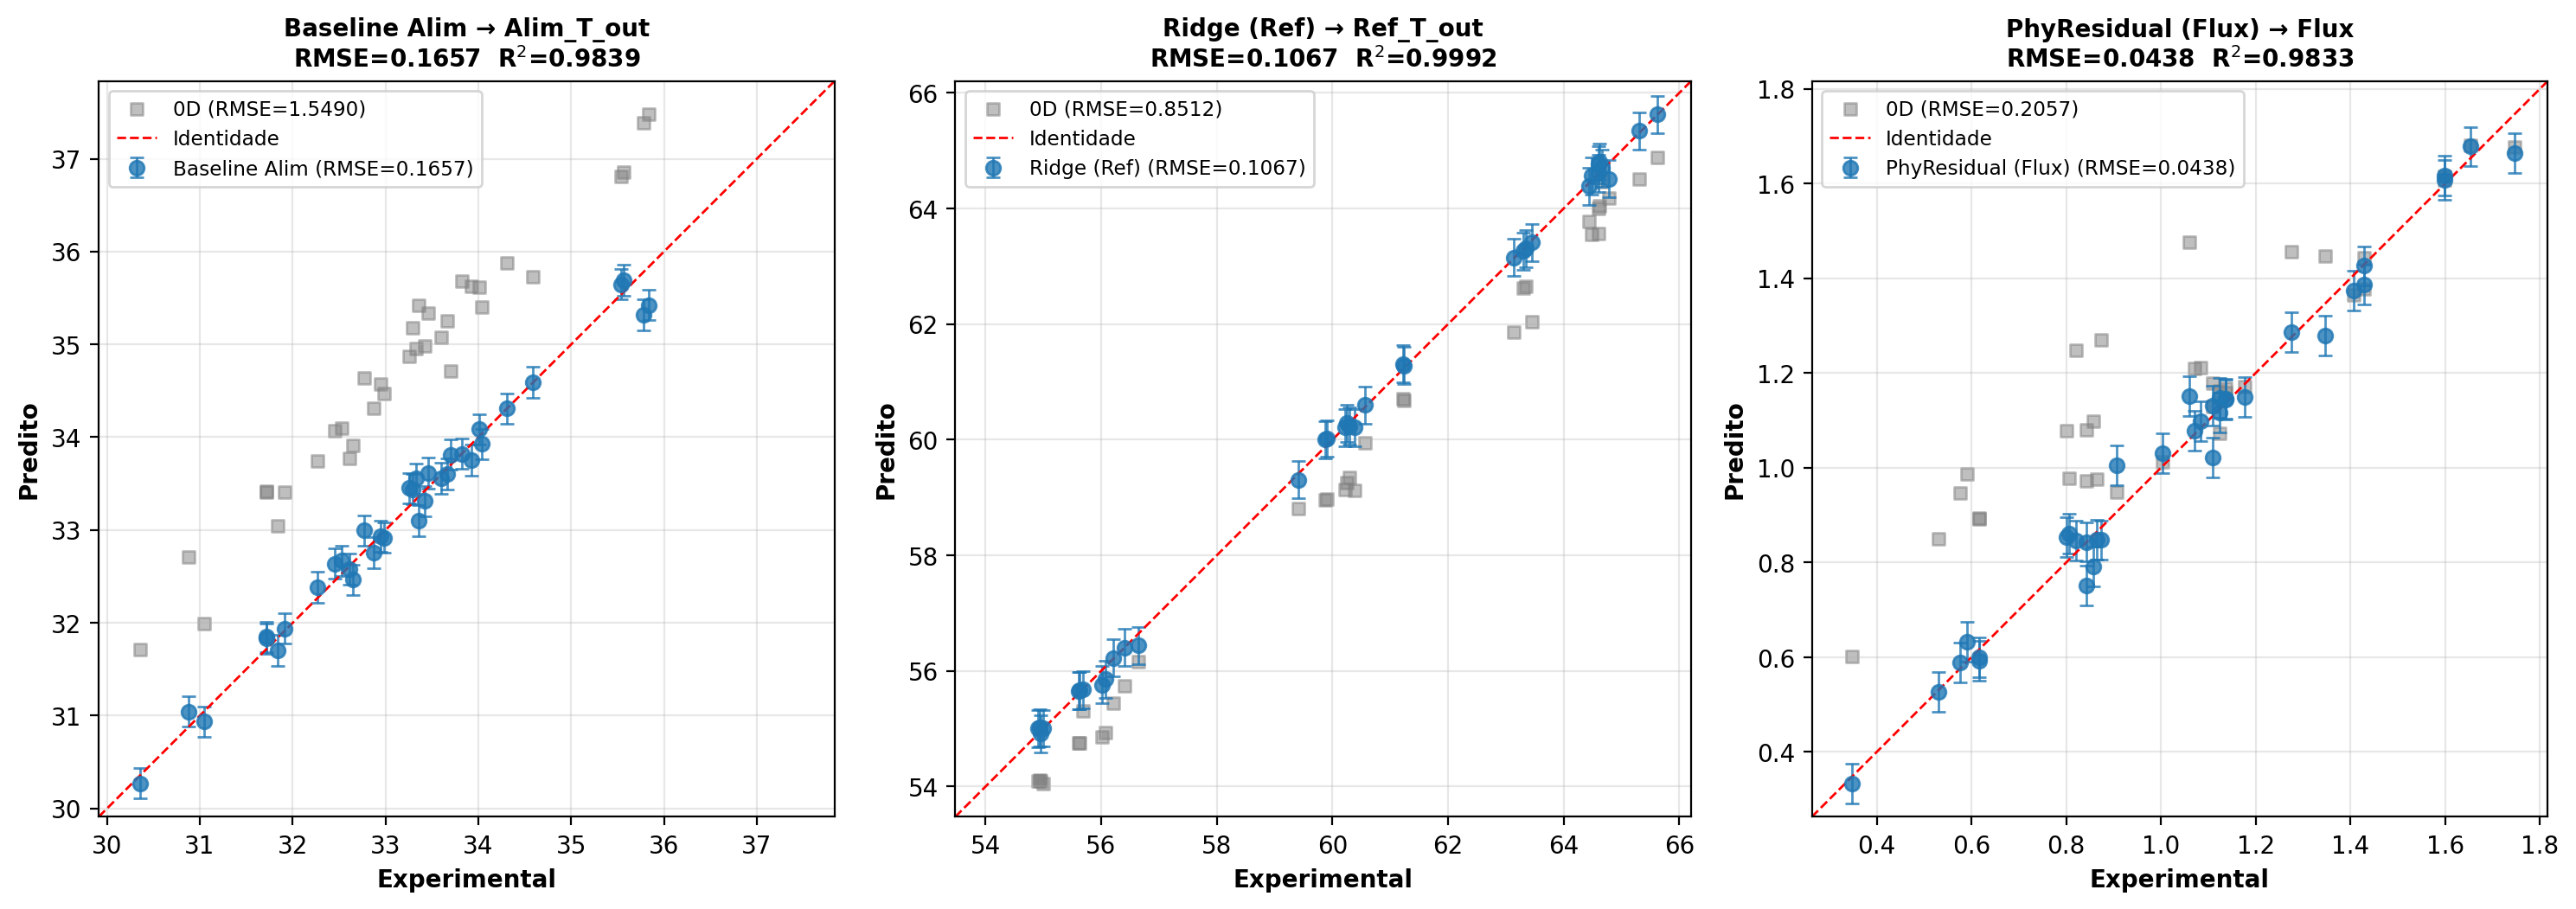
\includegraphics[width=0.85\textwidth]{tcc_images/chap06/model_selection/overlay_champions_panel_v2.png} b
  \vfill
    {\scriptsize \textcolor{blue!70!black}{T$_{alim,out}$}: Baseline Flux (Stage 1) \;|\;
    \textcolor{orange!70!black}{T$_{ref,out}$}: PhyResidual$^{Flux}$ (Stage 2) \;|\;
    \textcolor{green!70!black}{Flux}: PhyResidual$^{Flux}$ (Stage 2)}
  \\
  {\scriptsize Quadrados cinza = modelo físico 0D}
  \note{Overlay com os modelos selecionados: Baseline Flux para T\_alim (Stage 1), PhyResidual (base Flux) para T\_ref e Flux (Stage 2). Quadrados cinza = modelo 0D. [~1 min]}
\end{slide}
%========================================================================

    	\section{Conclusões}

\begin{slide}{Desempenho por Variável de Saída}
  \scriptsize
  \begin{columns}
    \begin{column}{0.94\linewidth}
    \begin{Item}[0.12]
    \item[\textbf{Temperaturas:}] Tanto para T$_{alim,out}$ quanto para T$_{ref,out}$, o \textbf{PhyResidual (Flux)} (Stage 2) obteve o menor Test RMSE (0,183 e 0,214, respectivamente). Para T$_{ref,out}$, a diferença sobre o Ridge (0,219) é marginal (2,3\%), mas o Ridge apresenta CV RMSE (0,195) muito inferior ao PhyResidual (0,346), indicando melhor generalização para regimes não vistos.
    \item[\textbf{Flux}:] Principal demonstração mensurável da vantagem da hibridização. \textbf{PhyResidual (Flux)} reduziu o RMSE em 73,8\% frente ao modelo 0D (0,206$\to$0,054). O R$^2$ passou de 0,951 (Stage 0) para 0,979, confirmando que a arquitetura residual extraiu maior poder preditivo ao incorporar a física como informação auxiliar.
    \item[\textbf{Resumo:}] Pelo critério puro de Test RMSE, o PhyResidual (base Flux) foi o melhor modelo para todas as três saídas. Para T$_{ref,out}$, modelos lineares são alternativas mais robustas para extrapolação, conectando-se com estratégias de correção linear multiplicativa na literatura.
    \end{Item}
    \end{column}
  \end{columns}
  \note{Flux: principal demonstração da hibridização (73,8\% melhor que 0D). Temperaturas: PhyResidual vence por Test RMSE, lineares têm melhor CV. [~2 min]}
\end{slide}
%========================================================================

\begin{slide}{Hibridização e Generalização}
  \footnotesize
  \begin{columns}
    \begin{column}{0.94\linewidth}
    \begin{Item}[0.12]
    \item A combinação do modelo físico 0D com redes neurais aproxima o cenário ideal de modelagem híbrida: unir o conhecimento da física aos dados experimentais.
    \item A arquitetura residual (PhyResidual) aprende o \textbf{viés} do modelo 0D (ex.: o erro sistemático de +1,58\,°C em T$_{alim,out}$) e calcula \textbf{apenas a correção residual}. Isso permite que a rede se concentre em ajustar o desvio entre a física simplificada e o comportamento real, sem precisar reaprender as relações físicas que o modelo 0D já representa adequadamente.
    \item Consequentemente, o PhyResidual preserva o \textbf{comportamento físico} do modelo 0D nas regiões onde sua variação está correta, e corrige apenas as discrepâncias para as características reais do sistema. Esse papel de \textbf{corretor de viés} é a principal contribuição mensurável da arquitetura residual para o fluxo de permeado: o RMSE caiu de 0,206 (0D) para 0,054 (PhyResidual), com R$^2$ de 0,979.
    \item Adicionalmente, o PhyResidual (Flux) manteve um erro estável sob regimes não vistos, com bom desempenho em relação às outras arquiteturas, tendo valores de CV RMSE comparáveis aos das regressões lineares para Flux (0,072 contra 0,082 do Lasso\_Indep). Para as temperaturas, no entanto, os modelos lineares apresentaram melhor CV RMSE (Ridge 0,195 para T$_{ref,out}$, OLS 0,196 para T$_{alim,out}$), sugerindo maior capacidade de extrapolação — direção que motiva a investigação de estratégias híbridas de correção linear multiplicativa (\cite{Villumsen2026}).
    \end{Item}
    \end{column}
  \end{columns}
  \note{Hibridização: residual aprende viés, preserva física, corrige dados reais. Flux: 0,206$\to$0,054 (74\% melhor). [~1,5 min]}
\end{slide}
%========================================================================

\begin{slide}{Trabalhos Futuros}
  \begin{Item}
    \item Substituir modelo 0D pelo modelo 2D (GITT) de \cite{Curcino2026} como referência física nas arquiteturas híbridas, aproveitando sua capacidade de capturar efeitos distribuídos
    \item Construir PINNs a partir das EDOs do modelo GITT — tanto como \textbf{surrogate} (apenas física, sem dados) para aceleramento de processamento, quanto no modo que incorpora dados experimentais na função de perda
    \item Investigar estratégias de correção linear multiplicativa (\cite{Villumsen2026}) como alternativa para melhor extrapolação: aplicar termo de correção linear sobre o modelo 0D/GITT, preservando consistência física mesmo sob regimes não vistos
  \end{Item}
  \note{Trabalhos futuros: modelo 2D GITT como referência física, PINNs a partir das EDOs, correção linear multiplicativa (Villumsen) para extrapolação. [~1,5 min]}
\end{slide}
%========================================================================


%% -------------------------------------------------
% Referências
%% -------------------------------------------------

\section{Referências Bibliográficas}
\label{sec:referencias}
\begin{slideWithFrameBreaks}{Referências Bibliográficas}
%\bibliographystyle{abntex2-alf.bst}
\bibliography{references/bibFile}
\scriptsize
\end{slideWithFrameBreaks}


%% -------------------------------------------------
% Slide de finalização
%% -------------------------------------------------
\begingroup
\usebackgroundtemplate
{
    \tikz\node[opacity=1]{
    %\includegraphics[height=\paperheight, width=\paperwidth]{}
    };
}
\setbeamertemplate{headline}{}
\setbeamertemplate{footline}{}
% \defbeamertemplate*{background canvas}{final}
% {%
%   \color{poliBlue}\vrule width\paperwidth height\paperheight% added bg color
% }
\begin{frame}{}

	
	\begin{center}
		

		
		\vspace{0.5cm}
		
		
\includegraphics[scale =.4]{figures/logo/Logo_EPUFRJ_2020.png}
		
		\vspace{0.3cm}
		

\begin{columns}
    \begin{column}{0.33\textwidth}

    \end{column}
    
    \begin{column}{0.34\textwidth}
    \centering
    %\color{poliRed!70!black}
    %\textbf{OBRIGADO!}

    \end{column}    
    
    \begin{column}{0.33\textwidth}
    

    \end{column}
\end{columns}
		
		
	\end{center}

	
\end{frame}
\endgroup
%% -------------------------------------------------
% Apêndice
%% -------------------------------------------------
%     \input{generalFormat/HeadAndFootAppendix}
%     \appendix 
%     \input{chapters/apendice1}
% %----------------------------------------------

\end{document}\usepackage[T1]{fontenc}